\documentclass[a4paper,twocolumn]{oblivoir}
\usepackage{amsmath,amssymb,kotex,kswrapfig,mdframed,paralist,graphicx}
\usepackage{fapapersize}
%\usefapapersize{210mm,297mm,10mm,*,10mm,*}

\usepackage{tabto,pifont}
%\TabPositions{0.1\textwidth,0.2\textwidth,0.3\textwidth,0.4\textwidth}
\newcommand\taba[5]{\par\noindent
\ding{172}\:{\ensuremath{#1}}
\tabto{0.1\textwidth}\ding{173}\:\:{\ensuremath{#2}}
\tabto{0.2\textwidth}\ding{174}\:\:{\ensuremath{#3}}
\tabto{0.3\textwidth}\ding{175}\:\:{\ensuremath{#4}}
\tabto{0.4\textwidth}\ding{176}\:\:{\ensuremath{#5}}}

\newcommand\tabb[5]{\par\bigskip\noindent
\ding{172}\:\:{\ensuremath{#1}}
\tabto{0.16\textwidth}\ding{173}\:\:{\ensuremath{#2}}
\tabto{0.33\textwidth}\ding{174}\:\:{\ensuremath{#3}}\medskip\par\noindent
\ding{175}\:\:{\ensuremath{#4}}
\tabto{0.16\textwidth}\ding{176}\:\:{\ensuremath{#5}}}

\newcommand\tabc[5]{\par\bigskip\noindent
\ding{172}\:\:{\ensuremath{#1}}
\tabto{0.25\textwidth}\ding{173}\:\:{\ensuremath{#2}}\medskip\par\noindent
\ding{174}\:\:{\ensuremath{#3}}
\tabto{0.25\textwidth}\ding{175}\:\:{\ensuremath{#4}}\medskip\par\noindent
\ding{176}\:\:{\ensuremath{#5}}}

\newcommand\tabd[5]{\par\bigskip\noindent
\ding{172}\:{\ensuremath{#1}}\medskip\par\noindent
\ding{173}\:\:{\ensuremath{#2}}\medskip\par\noindent
\ding{174}\:\:{\ensuremath{#3}}\medskip\par\noindent
\ding{175}\:\:{\ensuremath{#4}}\medskip\par\noindent
\ding{176}\:\:{\ensuremath{#5}}}

%
\newcommand\one{\ding{172}}
\newcommand\two{\ding{173}}
\newcommand\three{\ding{174}}
\newcommand\four{\ding{175}}
\newcommand\five{\ding{176}}


%\pagestyle{empty}

%%% Counters
\newcounter{num}
%\newcounter{answer}

%%% Commands
\newcommand\prob[1]
{\vs\par\noindent\refstepcounter{num} \textbf{문제 \thenum) #1}\par\noindent}

\newcommand\exam[1]
{\vs\par\noindent\refstepcounter{num} \textbf{예제 \thenum) #1}\par\noindent}

\newenvironment{expl}{\begin{mdframed}[frametitle=풀이]}{\end{mdframed}}

\newcommand\pb[1]{\ensuremath{\fbox{\phantom{#1}}}}

\newcommand\vs[1]{\vspace{30pt}}

\newcommand\an[1]{\par\bigskip\noindent\textbf{문제 \ref{#1})}\\}

\newcommand\ov[1]{\ensuremath{\overline{#1}}}

%%% Meta Commands
%\let\oldsection\section
%\renewcommand\section{\clearpage\oldsection}

\let\emph\textsf

\begin{document}
\title{중학교 3-1 기말 대비(천재교육 교과서)}
\date{\today}
\author{}
\maketitle

%%%
\section{이차방정식}

%
\prob{78}
\label{78}%4
\(A0\)용지는 반씩 계속 접어도 항상 닮은 모양이 된다고 한다.
다음 그림과 같이 반씩 접을 때마다 \(A1\), \(A2\), \(A3\), \(A4\), \(\cdots\)용지가 된다.
\(\overline{DE}=8\)이라고 할 때, \(\ov{DE}=8\)cm 이라고 할 때, \ov{PQ}의 길이를 구하여라.
(단, \(\square DEFG\)는 \(A0\)용지이다.)
\begin{center}
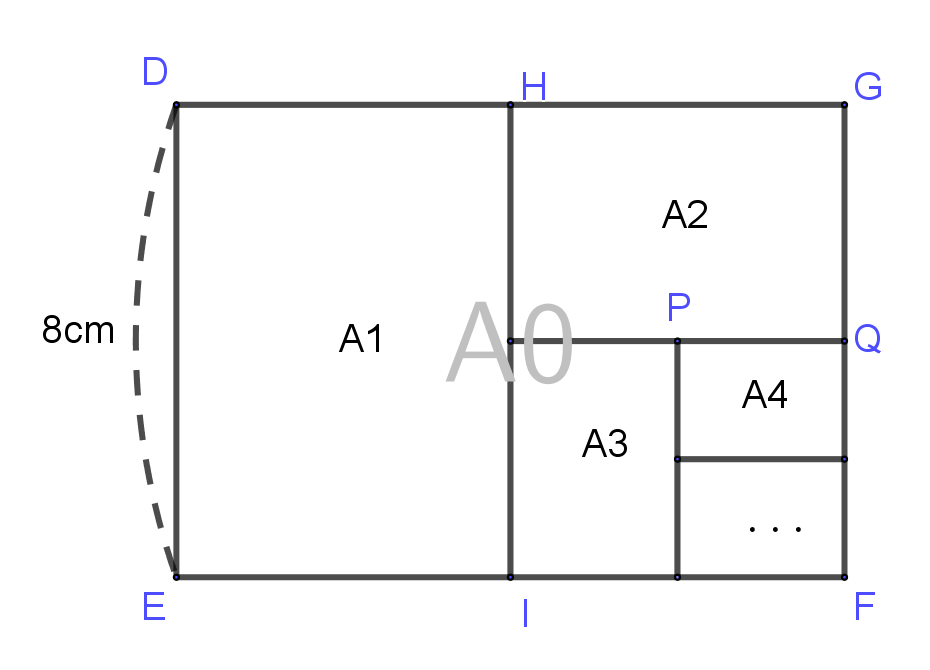
\includegraphics[width=0.35\textwidth]{78_1}
\end{center}
\taba1{\sqrt2}{2}{2\sqrt2}{4}

%
\prob{82-1}
\label{82-1}%2
한 개의 주사위를 던져서 나온 눈의 수가 이차방정식 \(x^2-6x+5=0\)의 해가 될 확률을 구하여라.
\taba{\frac16}{\frac13}{\frac12}{\frac23}{\frac56}

\newpage
%
\prob{82-2}\label{82-2}%1
한 개의 주사위를 던져서 나온 눈의 수가 이차방정식 \(2x^2-5x+2=0\)의 해가 될 확률을 구하여라.
\taba{\frac16}{\frac13}{\frac12}{\frac23}{\frac56}

%
\prob{82-3}\label{82-3}%3
한 개의 주사위를 던져서 나온 눈의 수가 이차방정식 \(|x-3|^2-4|x-3|+3=0\)의 해가 될 확률을 구하여라.
\taba{\frac16}{\frac13}{\frac12}{\frac23}{\frac56}


\prob{86-1}\label{86-1}%x=3
다음 마방진에서 가로, 세로, 대각선 방향에 있는 세 자연수의 합이 같다고 한다.
이 마방진이 \(2\)부터 \(10\)까지의 자연수로 이루어졌을 때, 조건에 알맞은 \(x\)의 값을 구하고 이 마방진을 완성하여라.
\begin{center}
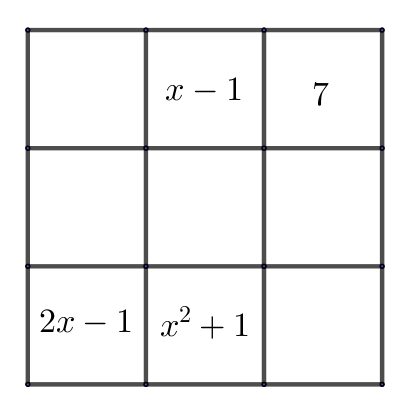
\includegraphics[width=0.2\textwidth]{86_1}
\end{center}

\newpage
%
\prob{86-2}\label{86-2}%x=2
마방진이 \(1\)부터 \(9\)까지의 자연수로 이루어졌을 때, 조건에 알맞은 \(x\)의 값을 구하고 이 마방진을 완성하여라.
\begin{center}
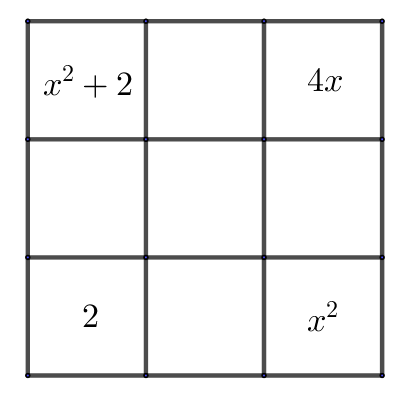
\includegraphics{86_2}
\end{center}

%
\prob{86-3}\label{86-3}%x=4
마방진이 \(6\)부터 \(14\)까지의 자연수로 이루어졌을 때, 조건에 알맞은 \(x\)의 값을 구하고 이 마방진을 완성하여라.
\begin{center}
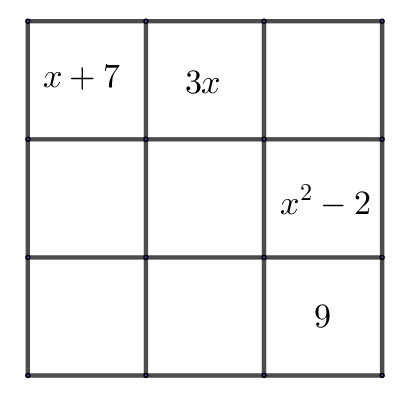
\includegraphics{86_3}
\end{center}

%
\prob{92-1}\label{92-1}%1
이차방정식 \(2x^2+4x+c=0\)이 중근을 가질 때 \(c\)의 값을 구하여라.
\taba23456

%
\prob{92-2}\label{92-2}%3
이차방정식 \(4x^2+bx+1=0\)이 중근을 가질 때 양의 실수 \(b\)의 값을 구하여라.
\taba23456

%
\prob{92-3}\label{92-3}%5
이차방정식 \(x^2+5x+c=0\)이 중근을 가질 때 \(c\)의 값을 구하여라.
\taba{\frac{21}4}{\frac{11}2}{\frac{23}4}6{\frac{25}4}

%
\prob{92-4}\label{92-4}%1
이차방정식 \(x^2+3x+c=0\)의 근이 유리수일 때, 자연수 \(c\)의 값을 구하여라.
\taba23456

%
\prob{92-5}\label{92-5}%2
이차방정식 \(7x^2-10x+c=0\)의 근이 유리수일 때, 자연수 \(c\)의 값을 구하여라.
\taba23456

%
\prob{92-6}\label{92-6}%5
이차방정식 \(x^2-5x+c=0\)의 근이 유리수일 때, 자연수 \(c\)의 최댓값을 구하여라.
\taba23456

%
\prob{98-1}\label{98-1}%2
리그전은 경기에 참가한 모든 팀이 서로 한 번씩 경기를 치르는 진행 방법을 말한다.
축구 경기를 리그전으로 치렀더니 총 \(55\)경기가 진행되었다.
이때 참가한 팀은 모두 몇 팀인가?
\taba{10}{11}{12}{13}{14}

%
\prob{98-2}\label{98-2}%4
어느 파티에 \(n\)명의 회원들이 초대되었다.
모든 회원들은 다른 모든 회원들과 한 번씩 악수를 했다.
총 \(78\)번의 악수가 이루어졌을 때 \(n\)의 값은?
\taba{10}{11}{12}{13}{14}

%
\prob{101-1}\label{101-1}%1
모양과 크기가 똑같은 카드 9장을 직사각형 모양으로 늘어놓았을 때, 직사각형 \(ABCD\)의 넓이가  \(810\text{cm}^2\)였다. 이때, 직사각형 \(ABCD\)의 둘레의 길이를 구하여라.
\begin{center}
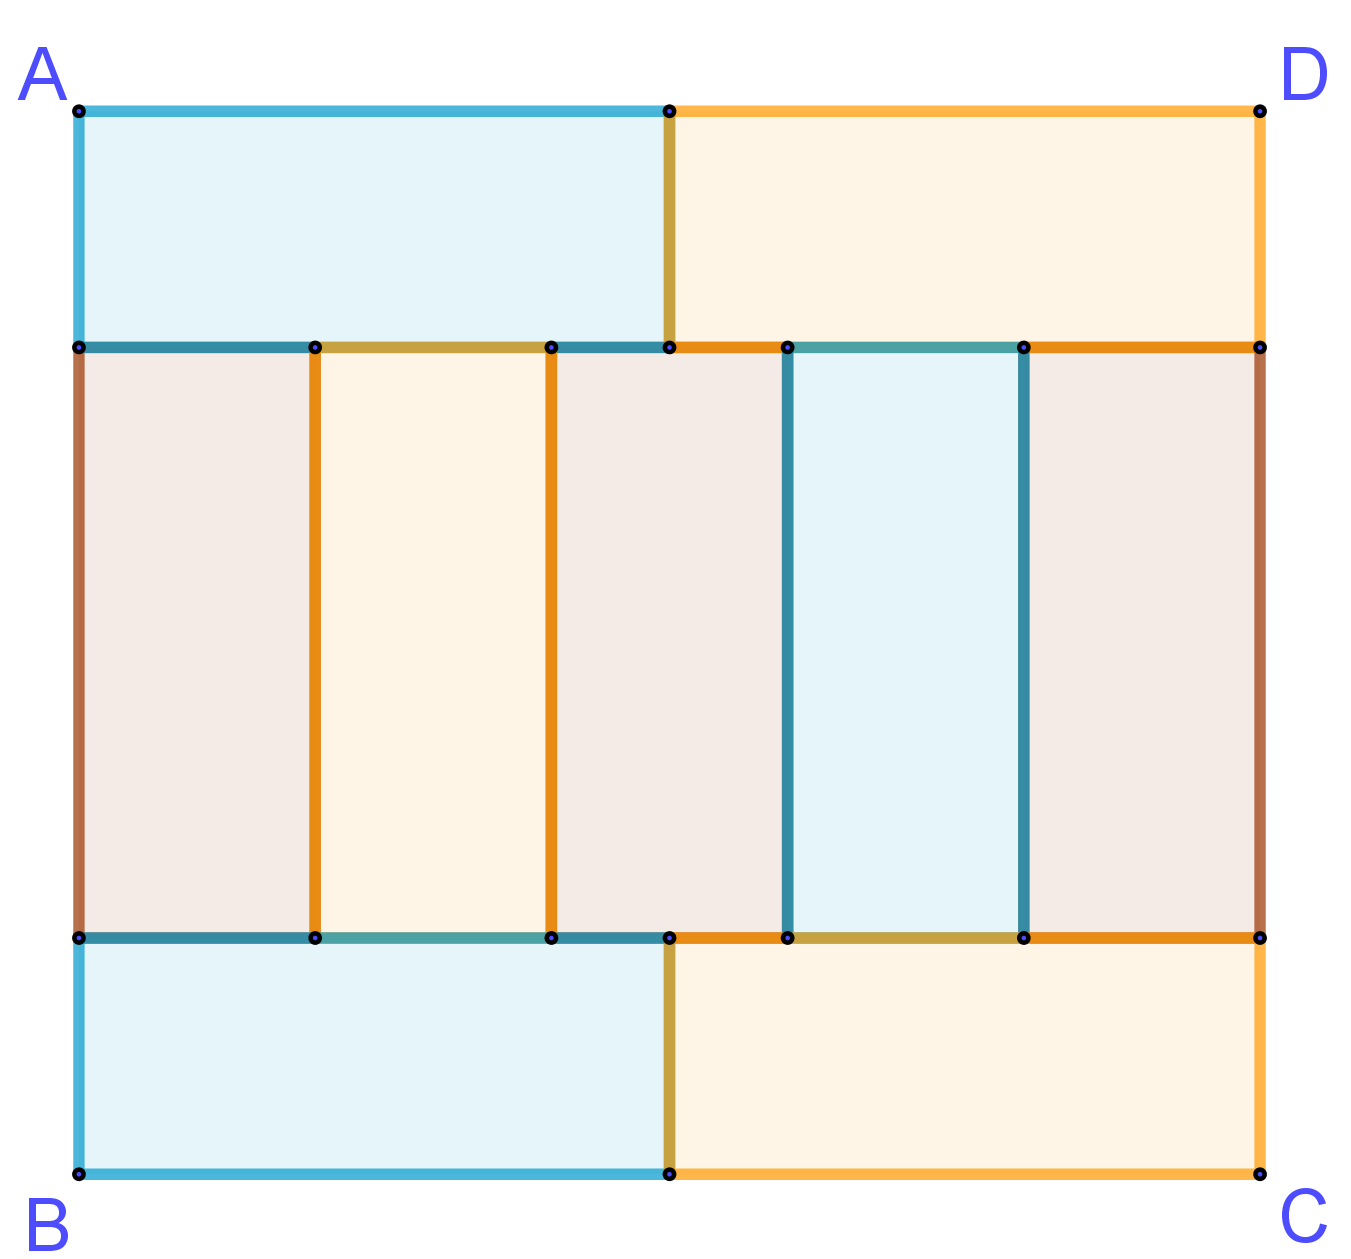
\includegraphics[width=0.4\textwidth]{101_1}
\end{center}
\taba{75\text{cm}}{88\text{cm}}{101\text{cm}}{114\text{cm}}{127\text{cm}}

%
\prob{101-2}\label{101-2}%4
모양과 크기가 똑같은 카드 10장을 직사각형 모양으로 늘어놓았을 때, 직사각형 \(ABCD\)의 넓이가  \(480\text{cm}^2\)였다. 이때, 직사각형 \(ABCD\)의 둘레의 길이를 구하여라.
\begin{center}
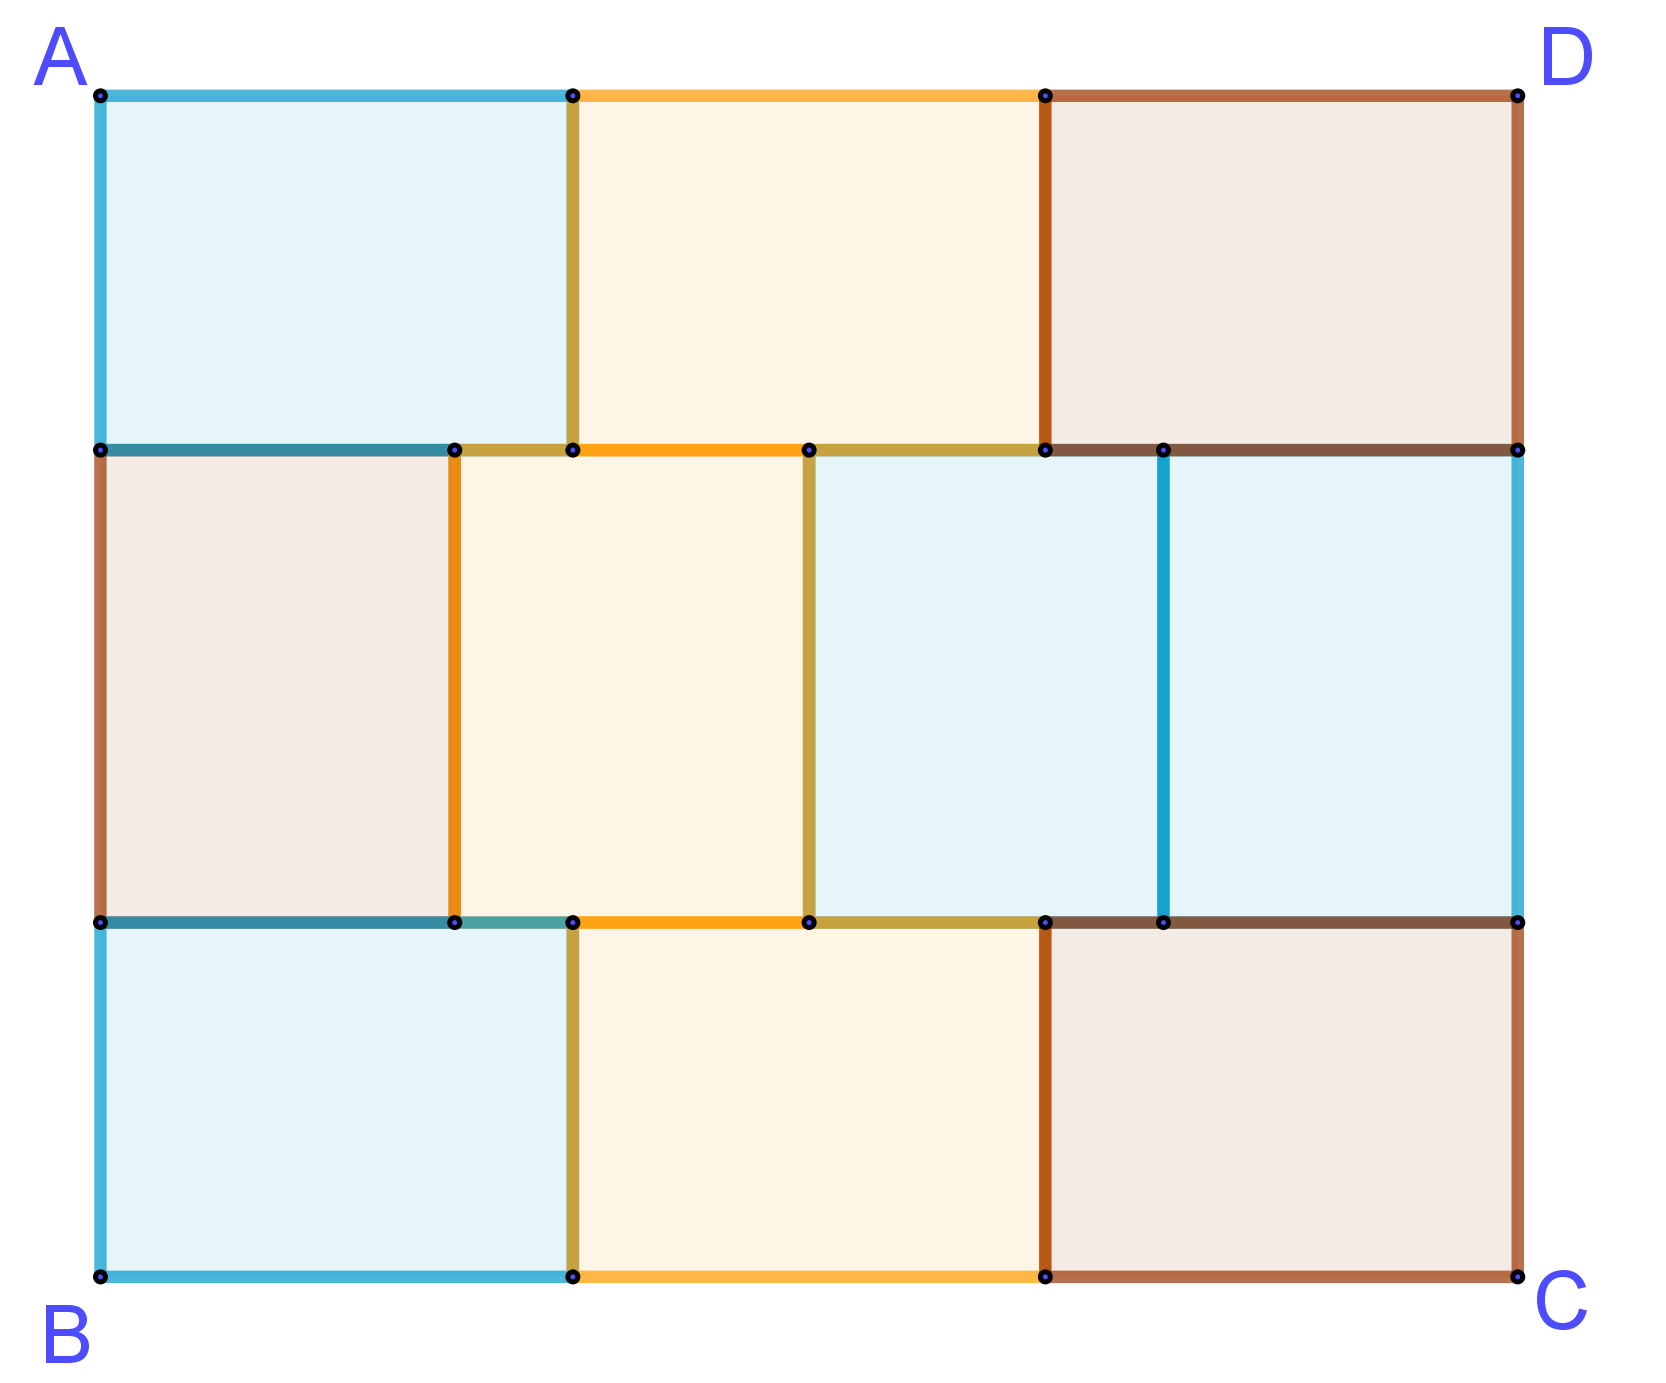
\includegraphics[width=0.4\textwidth]{101_2}
\end{center}
\taba{75\text{cm}}{88\text{cm}}{101\text{cm}}{114\text{cm}}{127\text{cm}}

\newpage
%
\prob{101-3}\label{101-3}%5
모양과 크기가 같은 직사각형 모양의 타일 6개를 넓이가 \(960\text{cm}^2\)인 직사각형 속에 빈틈없이 늘어 놓았더니 오른쪽 그림의 색칠한 부분과 같이 가로가 \(12\text{cm}\)인 직사각형 모양의 남는 부분이 생겼다.
이때, 타일의 짧은 변의 길이를 구하여라.
\begin{center}
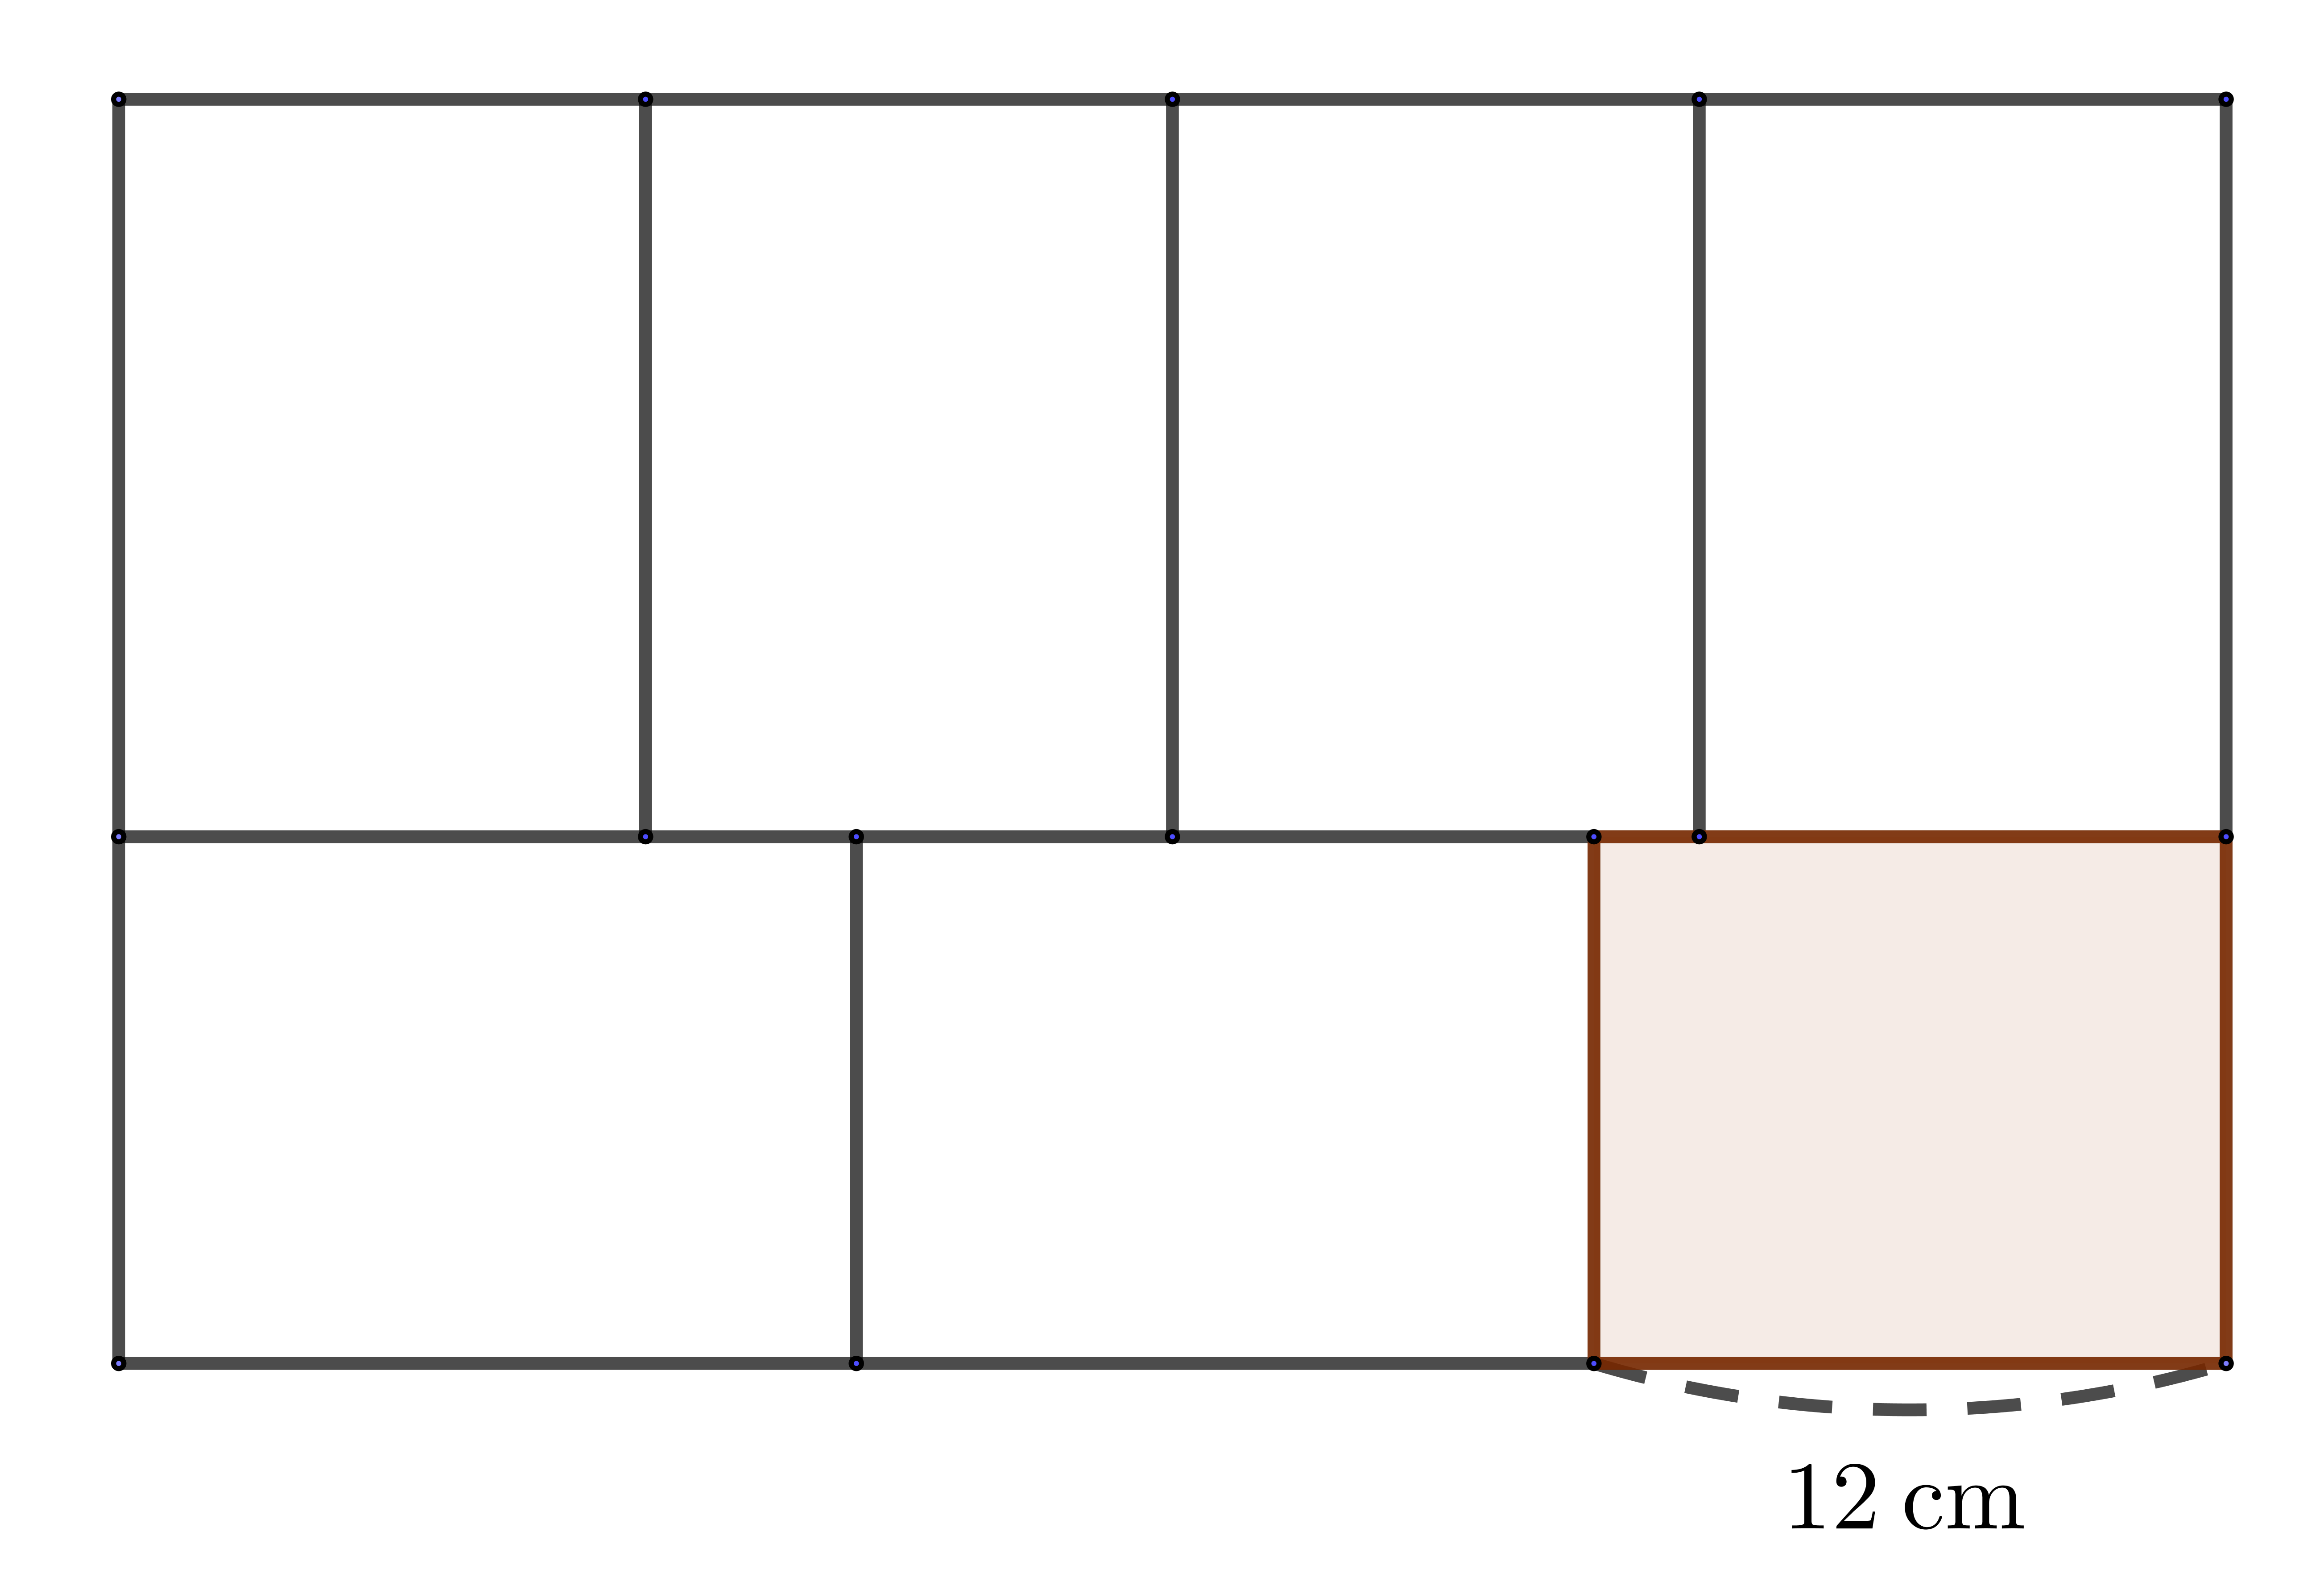
\includegraphics[width=0.4\textwidth]{101_3}
\end{center}
\taba{2\text{cm}}{4\text{cm}}{6\text{cm}}{8\text{cm}}{10\text{cm}}

%
\prob{101-4}\label{101-4}%2cm
직각삼각형 \(PQR\)의 넓이가 \(4\text{cm}^2\)일 때, \ov{PR}의 길이를 구하여라.
\begin{center}
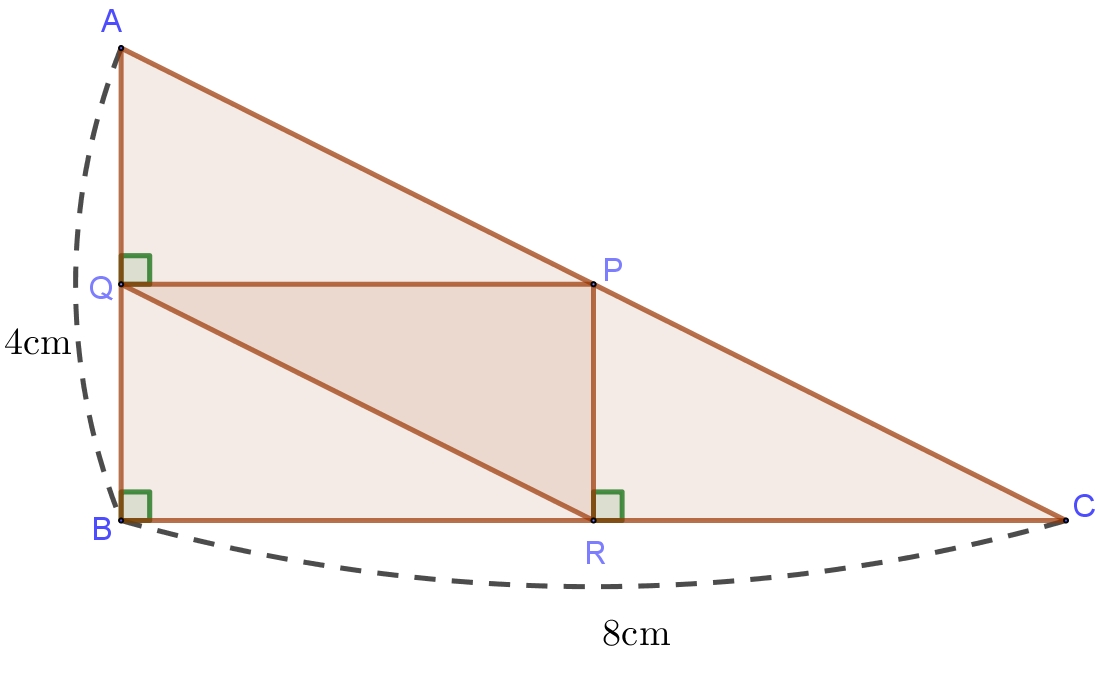
\includegraphics[width=0.4\textwidth]{101_4}
\end{center}
\taba{\frac12\text{cm}}{1\text{cm}}{\frac32\text{cm}}{2\text{cm}}{\frac32\text{cm}}

\newpage
%
\prob{101-5}\label{101-5}%3
직각삼각형 \(PQR\)의 넓이가 \(90\text{cm}^2\)일 때, \ov{PR}의 길이를 구하여라.
(단, \(\ov{PR}>\ov{PQ}\))
\begin{center}
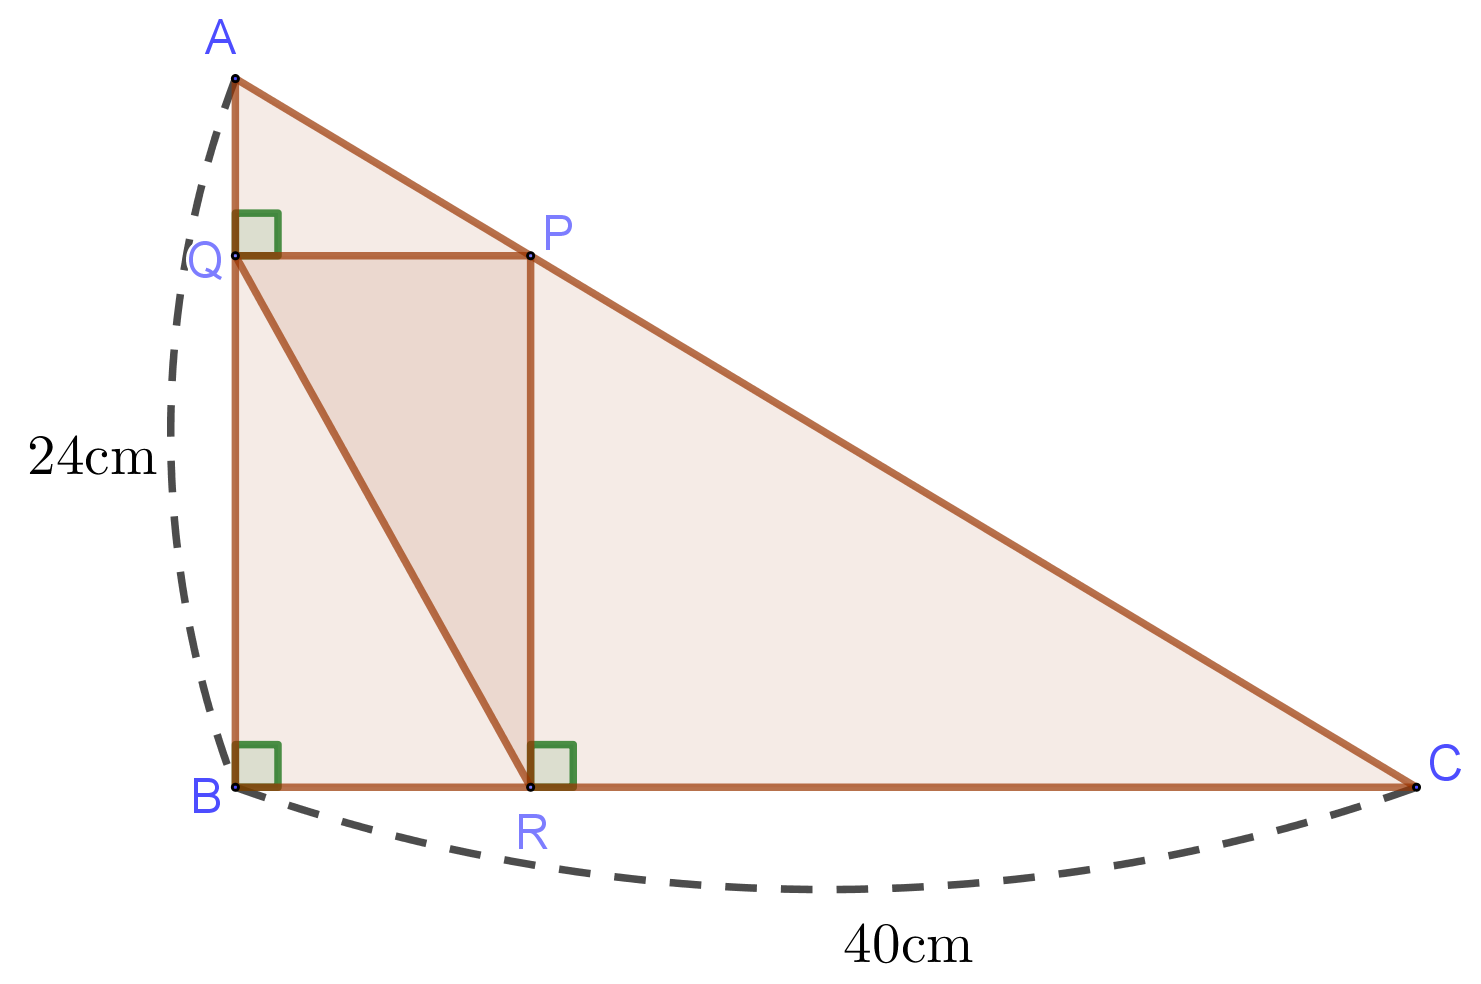
\includegraphics[width=0.4\textwidth]{101_5}
\end{center}
\taba{6\text{cm}}{12\text{cm}}{18\text{cm}}{24\text{cm}}{30\text{cm}}

\bigskip\bigskip\bigskip\bigskip
%\begin{mdframed}
\noindent
[문제 \ref{102-1})--문제 \ref{102-2}]\\
\fbox{다음과 같이 바둑돌을 나열할 때,\\ 물음에 답하여라.}
%\end{mdframed}

\begin{center}
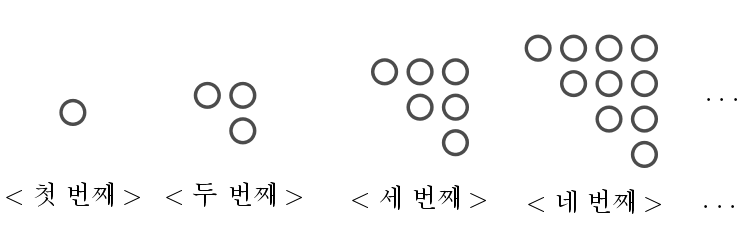
\includegraphics[width=0.45\textwidth]{102_1}
\end{center}

%
\prob{102-1}\label{102-1}%2
총 \(55\)개의 흰 바둑돌이 되는 것은 몇 번째인가?
\taba{10}{11}{12}{13}{14}

%
\prob{102-2}\label{102-2}%4
총 \(78\)개의 흰 바둑돌이 되는 것은 몇 번째인가?
\taba{10}{11}{12}{13}{14}

\newpage
%
\prob{103-1}\label{103-1}%4
직사각형 \(ABCD\)에서
점 \(P\)는 \ov{AB} 위를 점 \(A\)에서 점 \(B\)까지 1초에 \(1\)cm씩 움직이고,
점 \(Q\)는 \ov{BC} 위를 점 \(B\)에서 점 \(C\)까지 1초에 \(2\)cm씩 움직인다.
두 점 \(P\), \(Q\)가 동시에 출발할 때, \(\triangle PBQ\)의 넓이가 \(16\text{cm}^2\)이 될 때까지 걸리는 시간을 구하여라.
\begin{center}
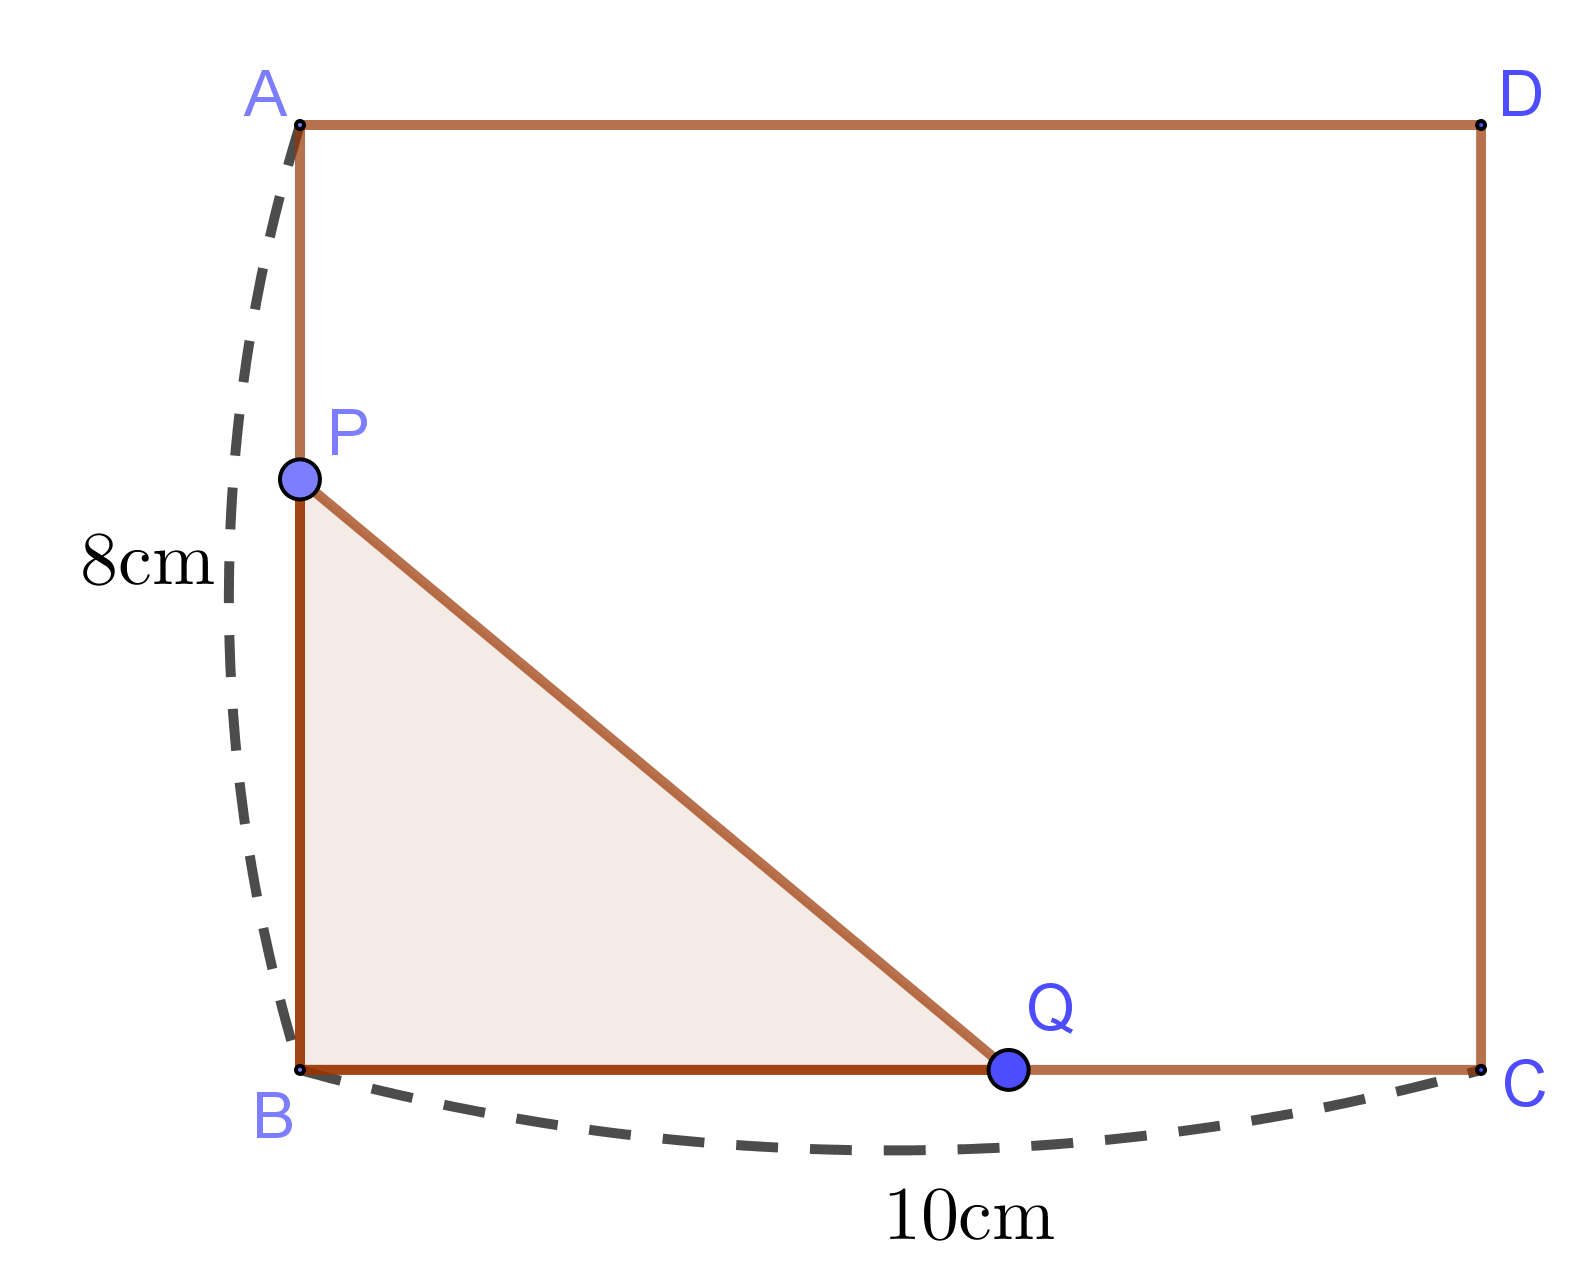
\includegraphics[width=0.4\textwidth]{103_1}
\end{center}
\taba{1초}{2초}{3초}{4초}{5초}

%
\prob{103-2}\label{103-2}%2
직사각형 \(ABCD\)에서
점 \(P\)는 \ov{AB} 위를 점 \(A\)에서 점 \(B\)까지 1초에 \(2\)cm씩 움직이고,
점 \(Q\)는 \ov{BC} 위를 점 \(B\)에서 점 \(C\)까지 1초에 \(3\)cm씩 움직인다.
두 점 \(P\), \(Q\)가 동시에 출발할 때, \(\triangle PBQ\)의 넓이가 처음으로 \(33\text{cm}^2\)이 될 때까지 걸리는 시간을 구하여라.
\begin{center}
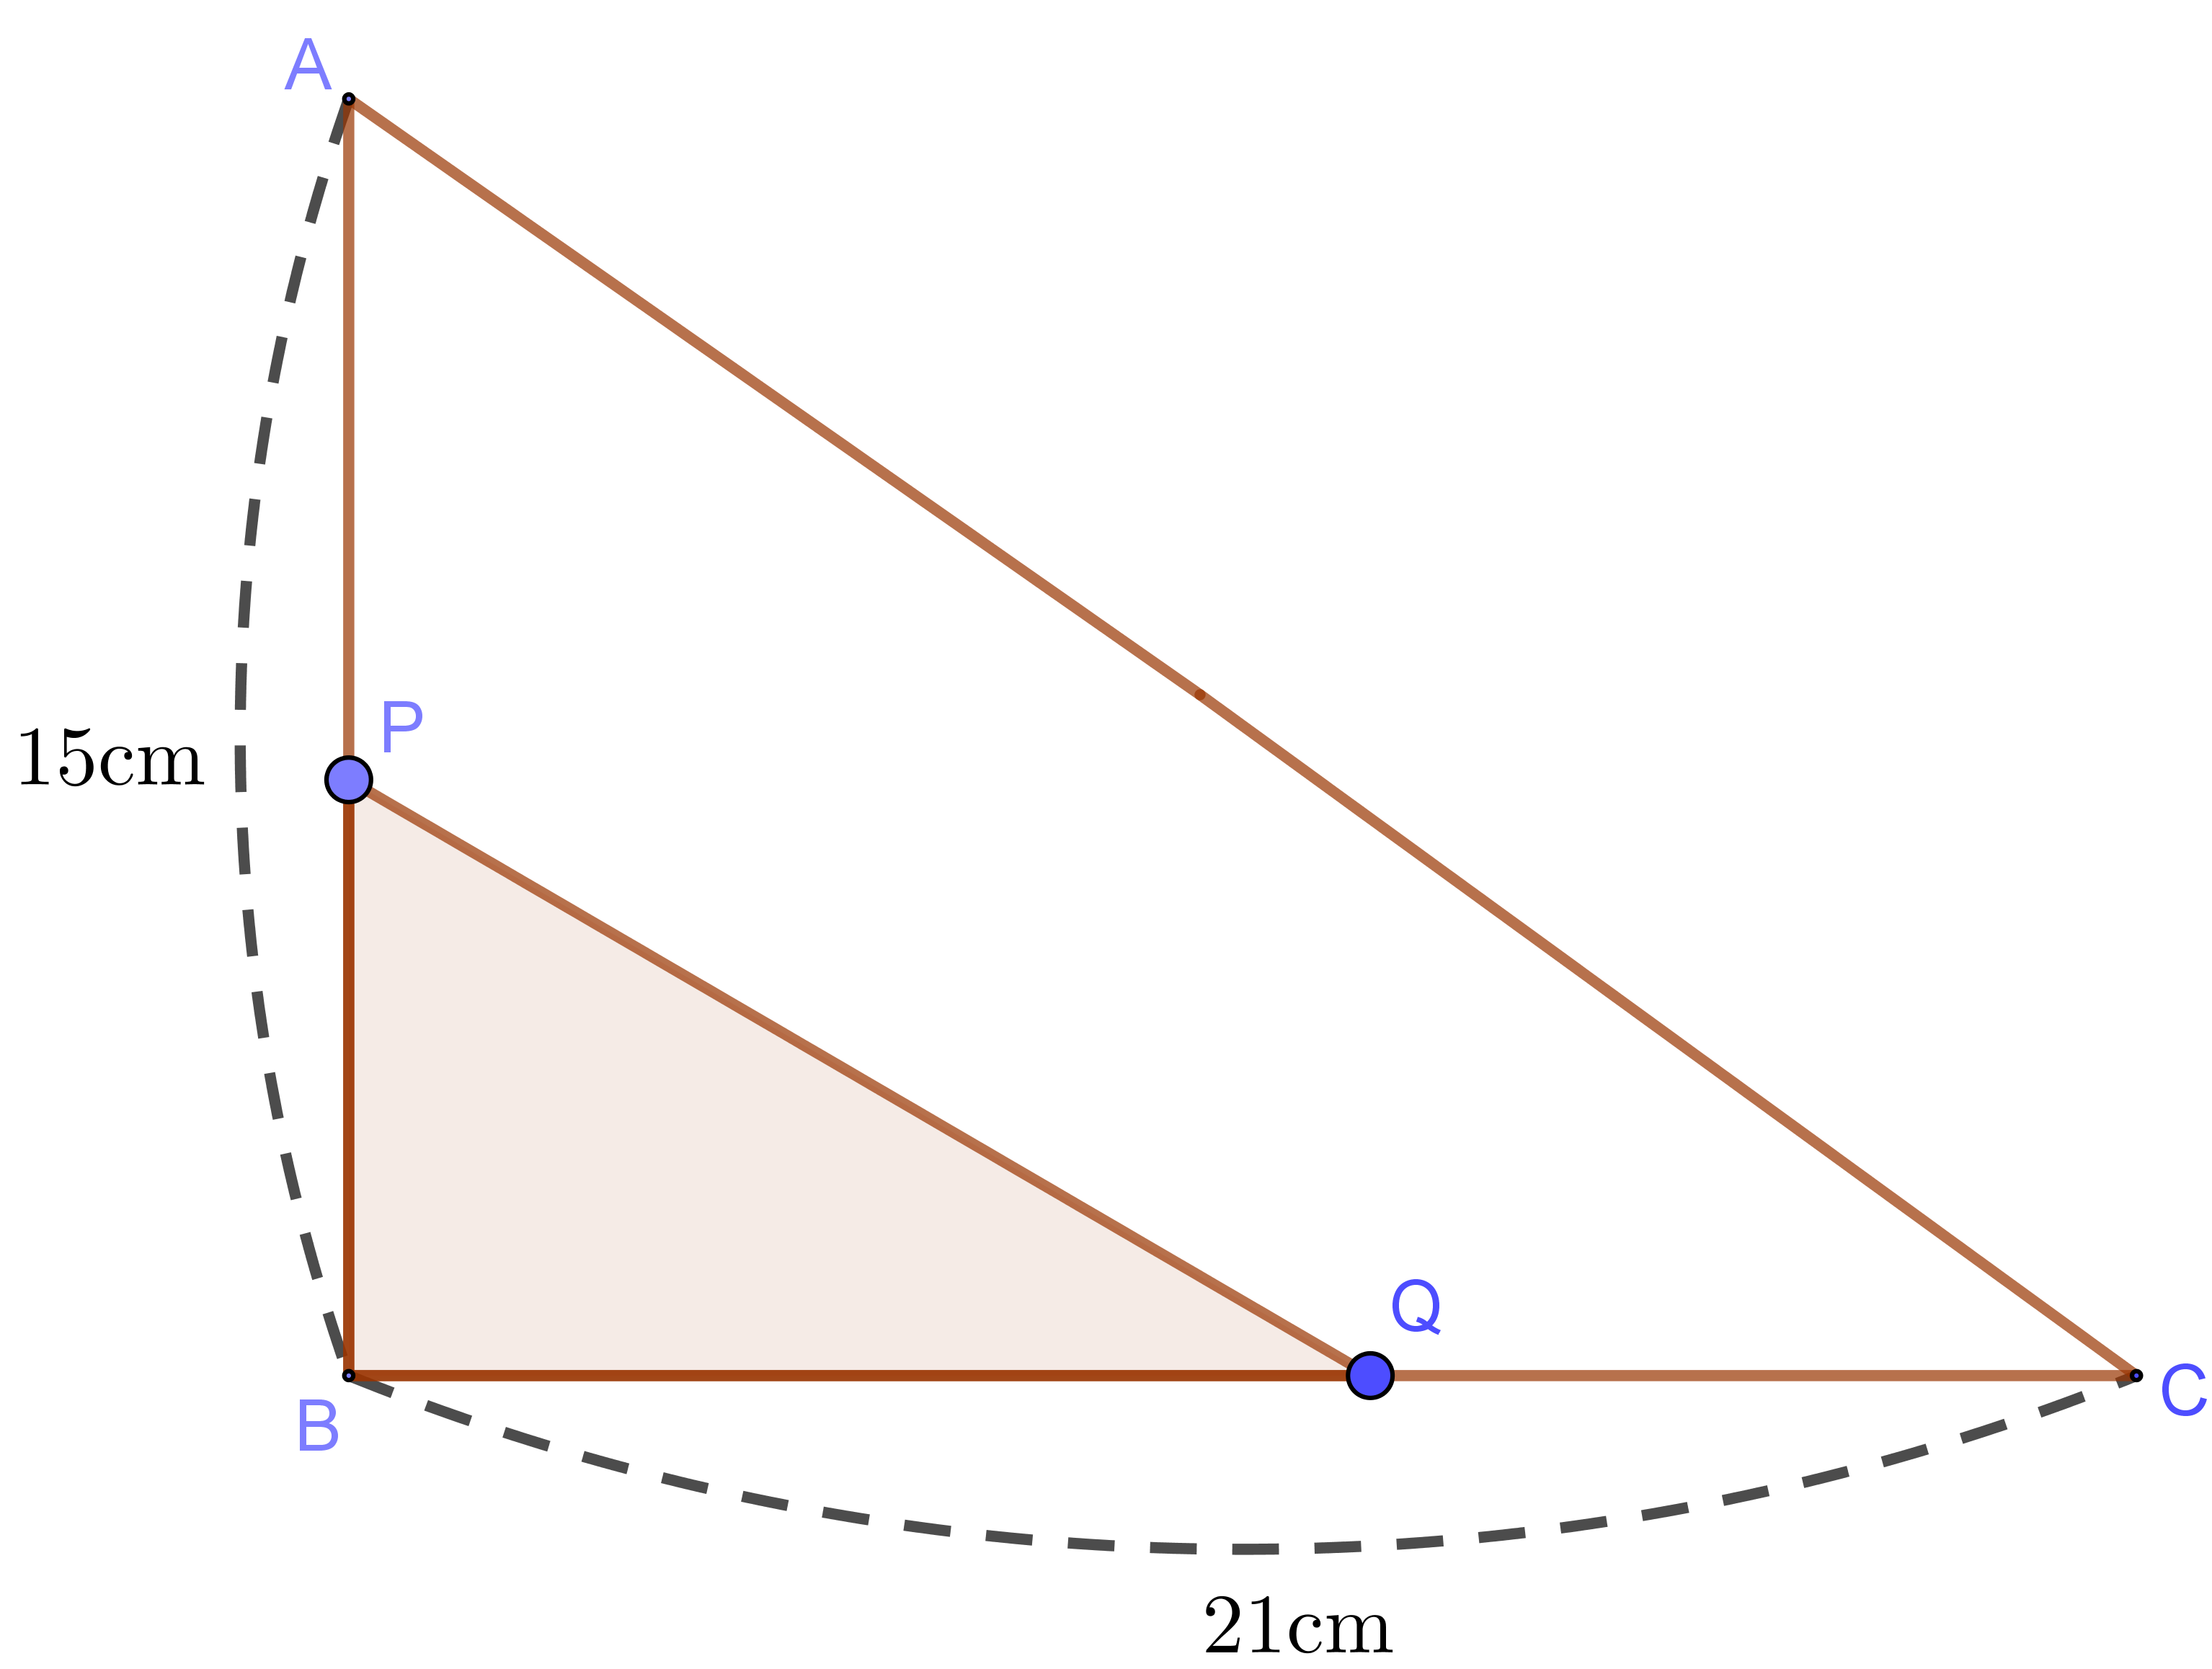
\includegraphics[width=0.4\textwidth]{103_2}
\end{center}
\taba{1초}{2초}{3초}{4초}{5초}

%
\prob{106-1}\label{106-1}%4
길이가 \(3\)m인 끈을 두 도막으로 잘라서 크기가 서로 다른 두 개의 정사각형을 만들려고 한다. 두 정사각형의 넓이의 비가 \(1:2\)일 때, 큰 정사각형의 한 변의 길이를 구하여라. 
\tabc
{\frac{6+3\sqrt2}2}{\frac{6-3\sqrt2}2}
{\frac{6+3\sqrt2}4}{\frac{6-3\sqrt2}4}
{\frac{2+\sqrt2}2}

%
\prob{106-2}\label{106-2}%1
길이가 \(5\)m인 끈을 두 도막으로 잘라서 크기가 서로 다른 두 개의 정사각형을 만들려고 한다. 두 정사각형의 넓이의 비가 \(1:3\)일 때, 큰 정사각형의 한 변의 길이를 구하여라.
\tabc
{\frac{15-5\sqrt3}8}{\frac{15-5\sqrt3}4}
{\frac{15-10\sqrt3}8}{\frac{15-10\sqrt3}4}
{\frac{15-15\sqrt3}8}

%
\prob{106-3}\label{106-3}%1
길이가 \(5\)m인 끈을 두 도막으로 잘라서 크기가 서로 다른 두 개의 정사각형을 만들려고 한다. 두 정사각형의 넓이의 비가 \(1:4\)일 때, 큰 정사각형의 한 변의 길이를 구하여라.
\taba{\frac65}{\frac75}{\frac85}{\frac95}{\frac{10}5}

\newpage
%
\prob{107-1}\label{107-1}%4
아래 그림에서 \(\ov{OD}=\ov{OF}\)이다.
사각형 \(CDEF\)의 작은 변의 길이를 \(a\), 큰 변의 길이를 \(b\)라고 할 때, \(\frac ba\)의 값을 구하여라.
\begin{center}
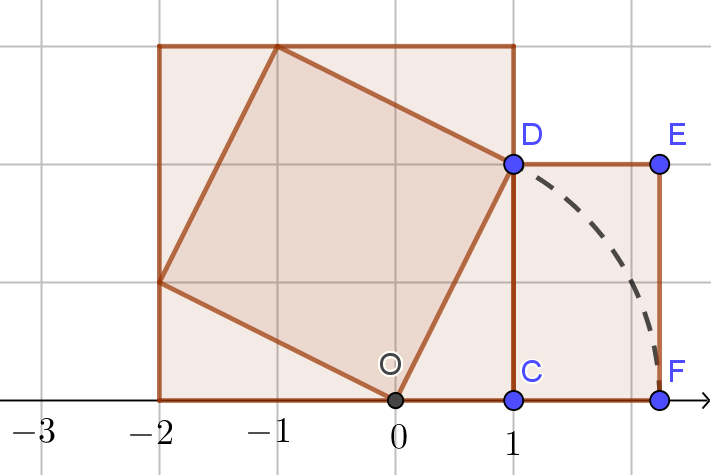
\includegraphics[width=0.35\textwidth]{107_1}
\end{center}
\tabb
{\frac{\sqrt3-1}2}{\frac{\sqrt3+1}2}{\frac{\sqrt5-1}2}{\frac{\sqrt5+1}2}{\frac{\sqrt6-1}2}

%
\prob{107-2}\label{107-2}%4
아래 그림에서 \(\square AEFD\)는 정사각형이고, 두 직사각형 \(ABCD\), \(BCFE\)는 서로 닮은 도형이다.
\(\ov{BC}=4\)일 때, \(\frac{\ov{AB}}{\ov{BC}}\)의 값을 구하여라.
\begin{center}
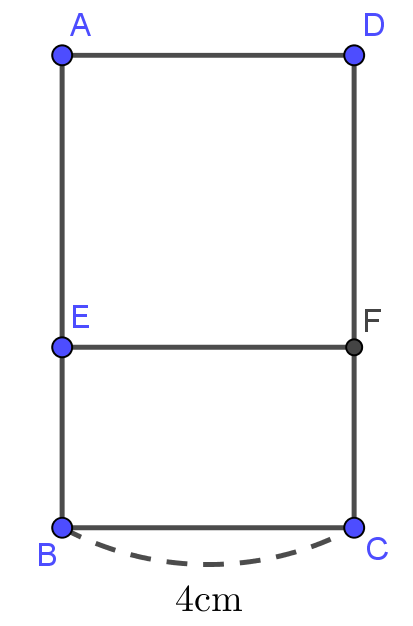
\includegraphics[width=0.2\textwidth]{107_2}
\end{center}
\tabb
{\frac{\sqrt3-1}2}{\frac{\sqrt3+1}2}{\frac{\sqrt5-1}2}{\frac{\sqrt5+1}2}{\frac{\sqrt6-1}2}

\newpage
%
\prob{107-3}\label{107_3}%4
아래 그림에서 \(\triangle ABC\)는 \(\ov{AB}=\ov{AC}=10\text{cm}\)인\\ 이등변삼각형이다.
\(\angle C=72^\circ\), \(\angle ABD=\angle CBD\)일 때, \(\frac{\ov{AB}}{\ov{BC}}\)의 값을 구하여라.
\begin{center}
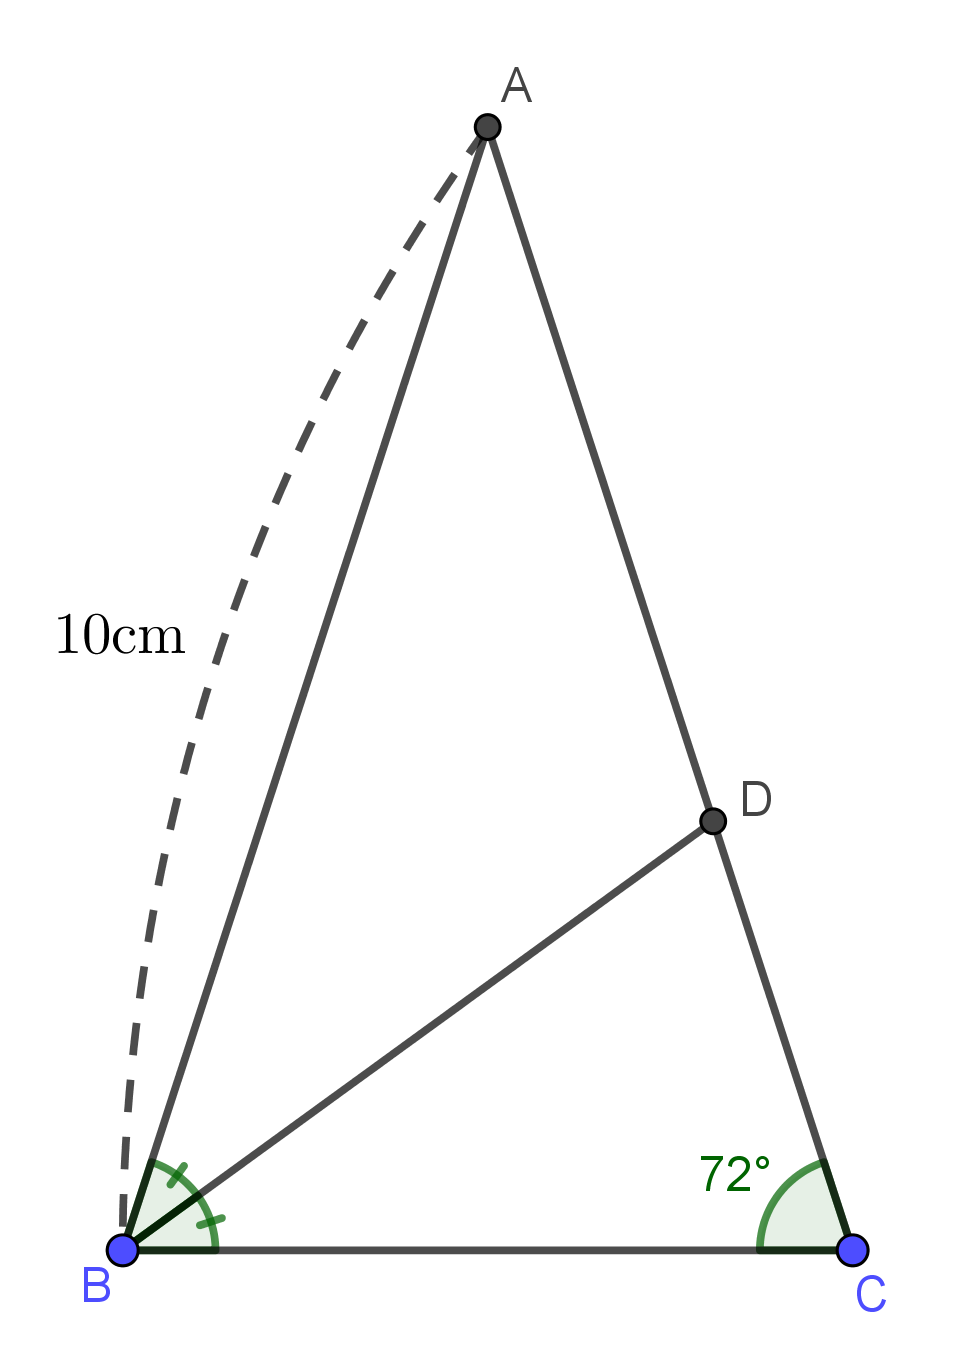
\includegraphics[width=0.2\textwidth]{107_3}
\end{center}
\tabb
{\frac{\sqrt3-1}2}{\frac{\sqrt3+1}2}{\frac{\sqrt5-1}2}{\frac{\sqrt5+1}2}{\frac{\sqrt6-1}2}
\vspace{10pt}

%%
\section{이차함수}

\vspace{-30pt}
%
\prob{123-1}\label{123-1}%3
전력 \(P\)와 전류 \(I\) 사이에는 \(P=I^2R\)의 관계가 있다고 한다.
전류의 변화에 따른 전력의 변화를 실험한 결과가 오른쪽 그림과 같을 때, 이 물체의 저항 \(R\)의 값을 구하여라.
\begin{center}
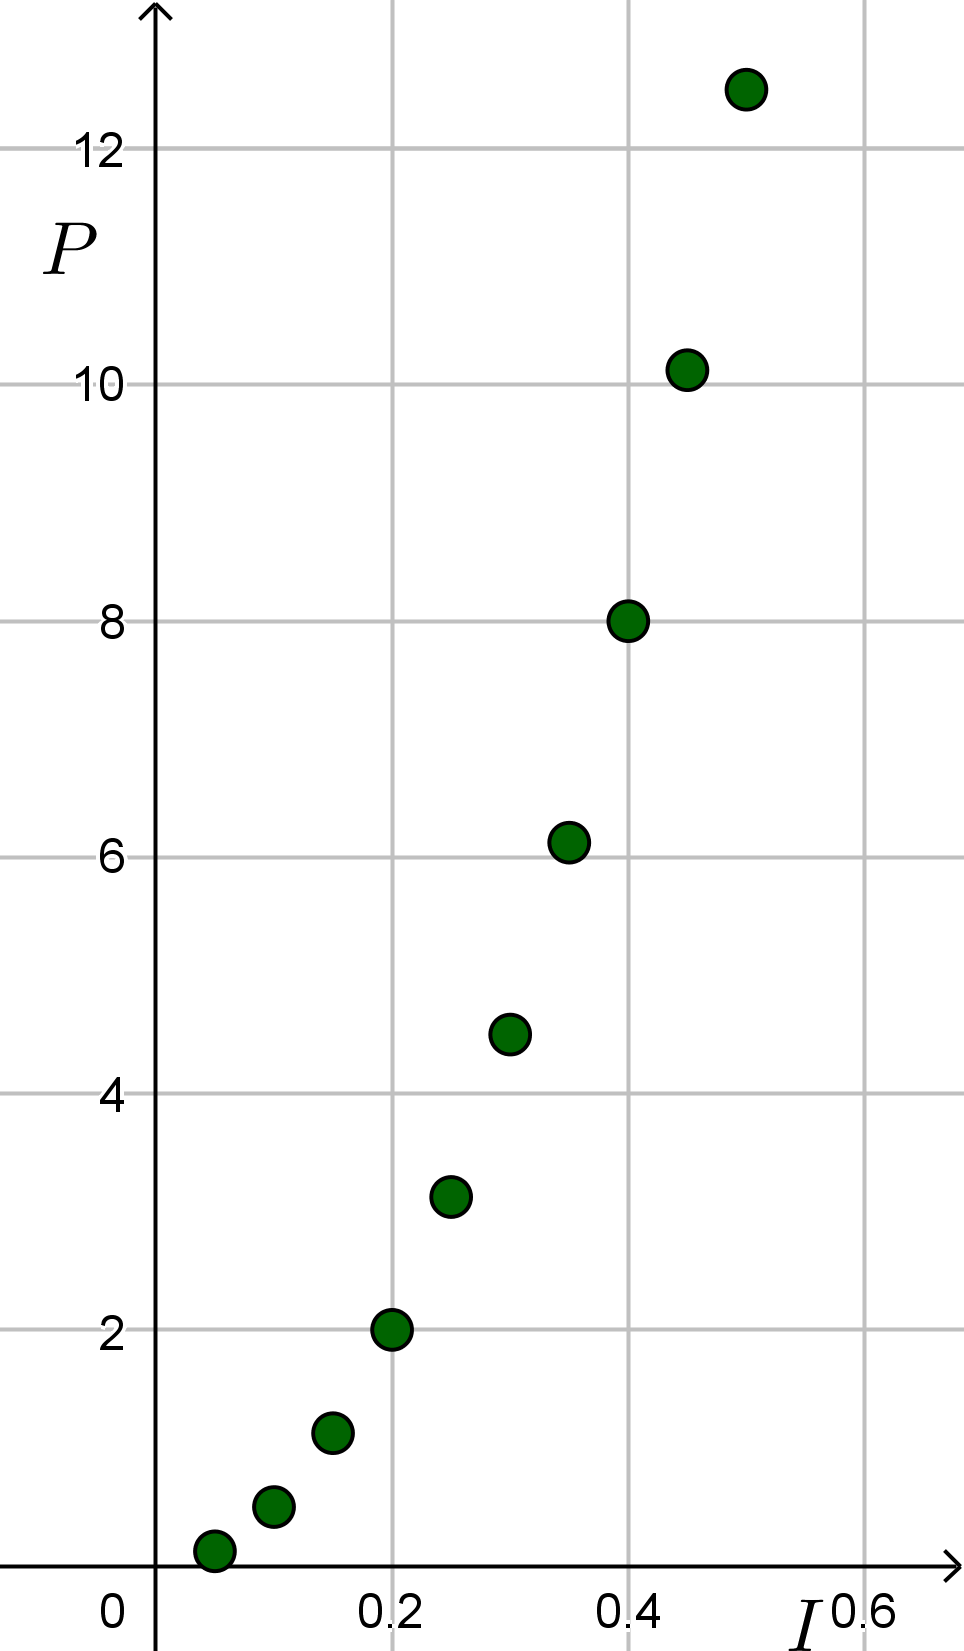
\includegraphics[width=0.17\textwidth]{123_1}
\end{center}
\taba{10}{25}{50}{75}{100}

\newpage
%
\prob{123-2}\label{123-2}%2
전력 \(P\)와 전류 \(I\) 사이에는 \(P=I^2R\)의 관계가 있다고 한다.
전류의 변화에 따른 전력의 변화를 실험한 결과가 오른쪽 그림과 같을 때, 이 물체의 저항 \(R\)의 값을 구하여라.
\begin{center}
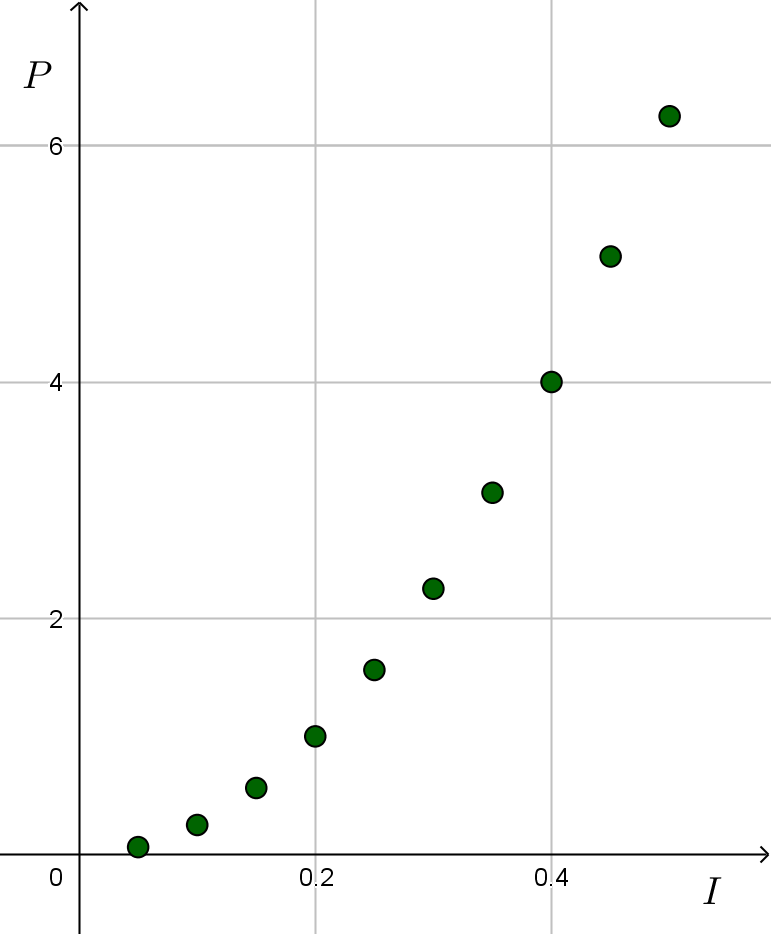
\includegraphics[width=0.2\textwidth]{123_2}
\end{center}
\taba{10}{25}{50}{75}{100}

%
\prob{123-3}\label{123-3}%1
전력 \(P\)와 전압 \(V\) 사이에는 \(P=\frac{V^2}R\)의 관계가 있다고 한다.
전압의 변화에 따른 전력의 변화를 실험한 결과가 오른쪽 그림과 같을 때, 이 물체의 저항 \(R\)의 값을 구하여라.
\begin{center}
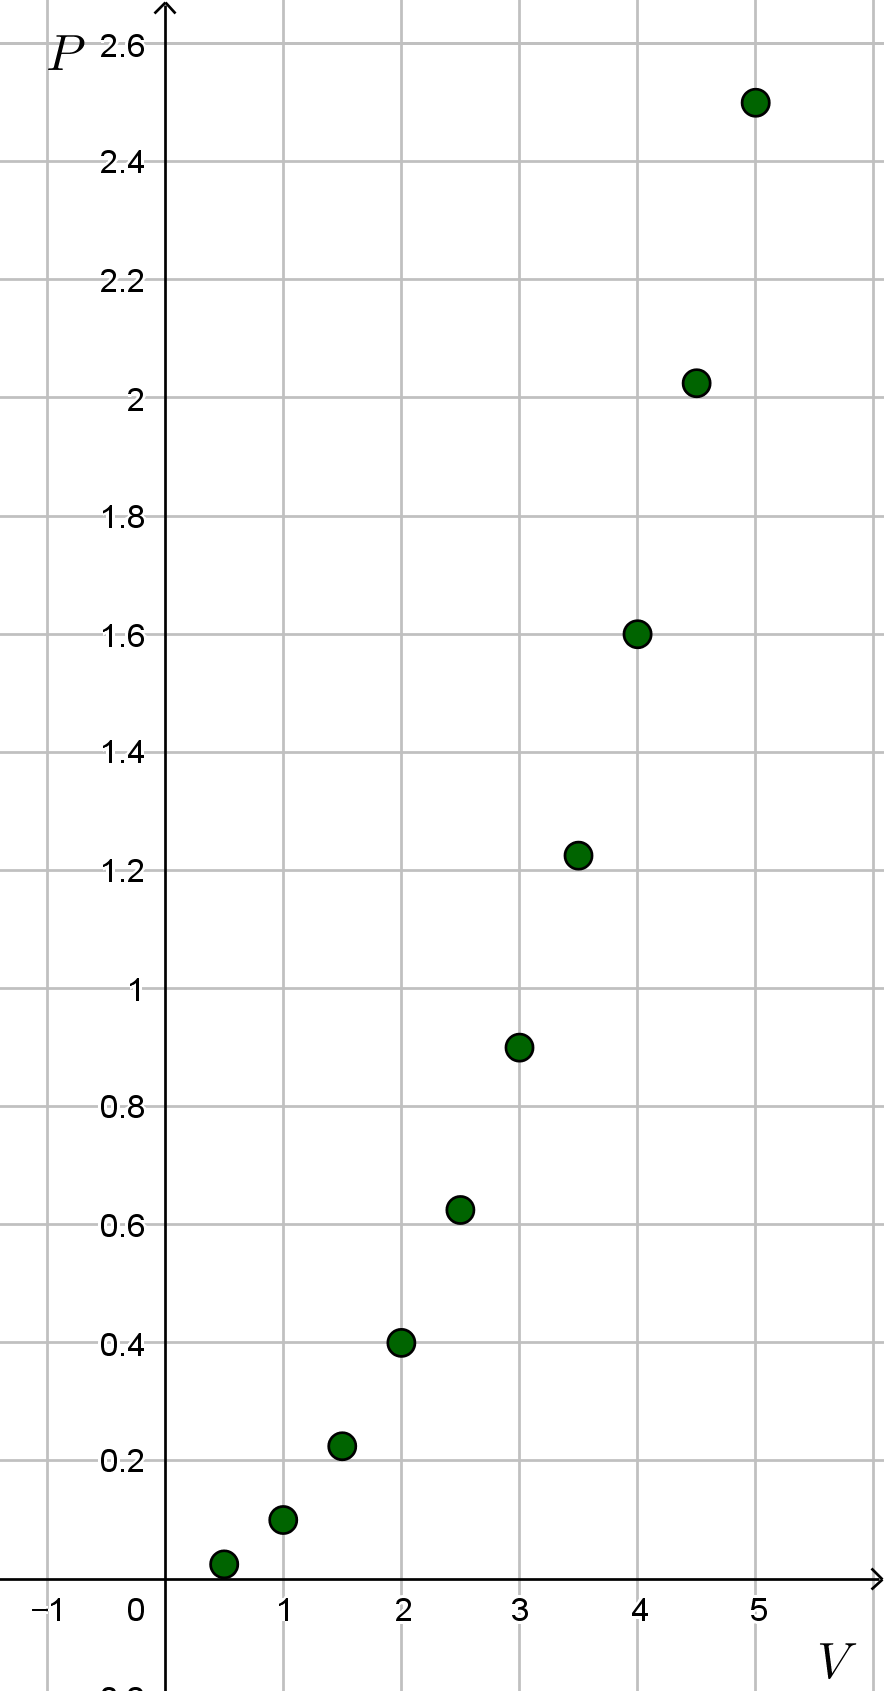
\includegraphics[width=0.22\textwidth]{123_3}
\end{center}
\taba{10}{25}{50}{75}{100}

\newpage
%
\prob{130-1}\label{130-1}%5
아래 그림에서 ⓐ, ⓑ는 각각 이차함수 \(y=x^2+2\)와 \(y=x^2-4\)의 그래프이다.
이때, 색칠한 부분의 넓이를 구하여라.
\begin{center}
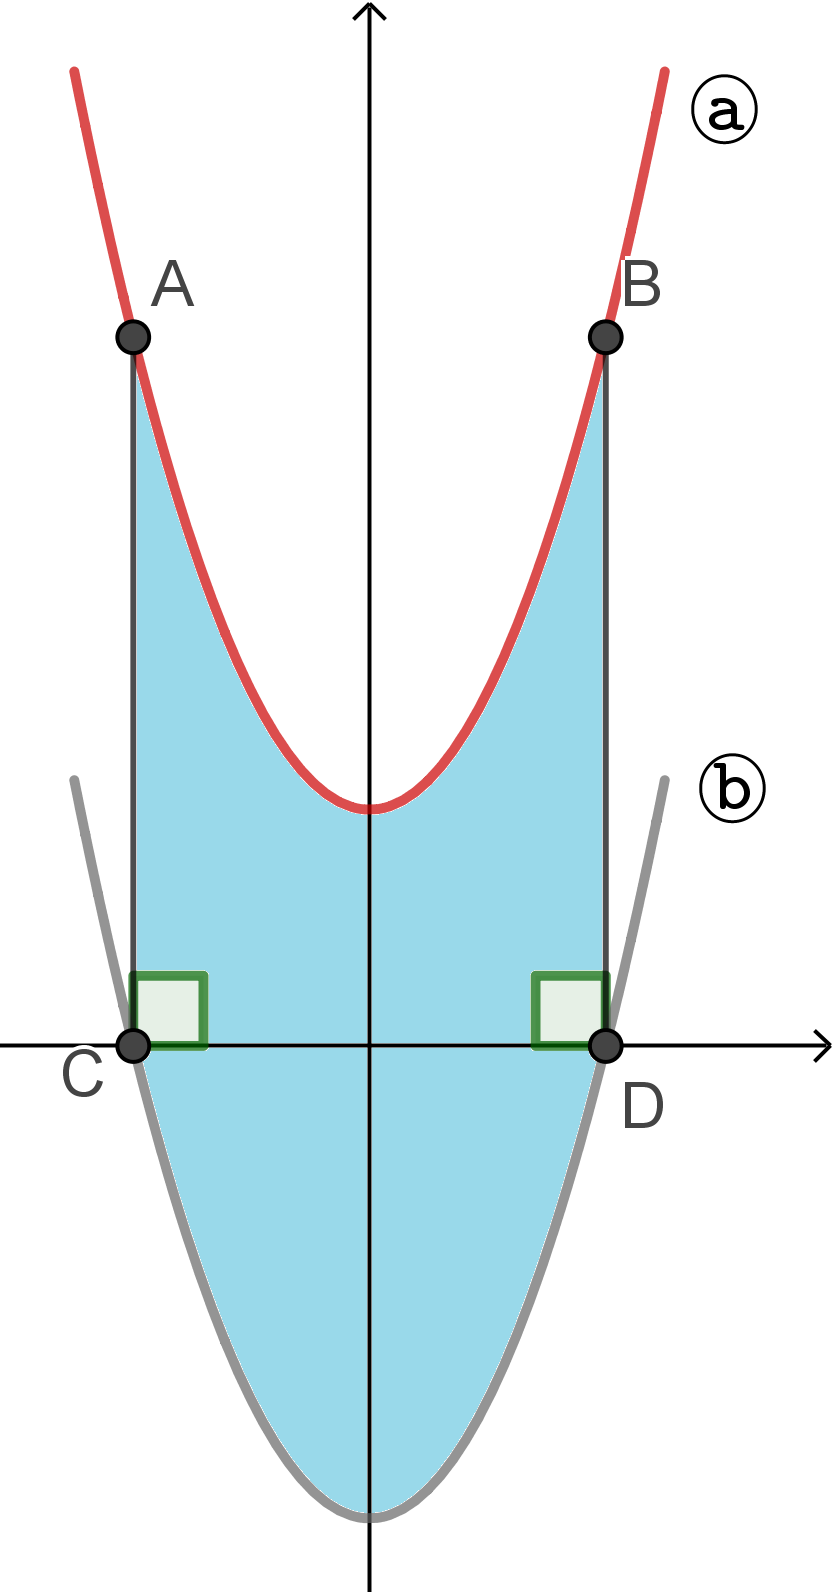
\includegraphics[width=0.23\textwidth]{130_1}
\end{center}
\taba8{12}{16}{20}{24}

%
\prob{130-2}\label{130-2}%5
아래 그림에서 ⓐ, ⓑ는 각각 이차함수 \(y=\frac12x^2+3\)와 \(y=\frac12 x^2-3\)의 그래프이다.
이때, 색칠한 부분의 넓이를 구하여라.
\begin{center}
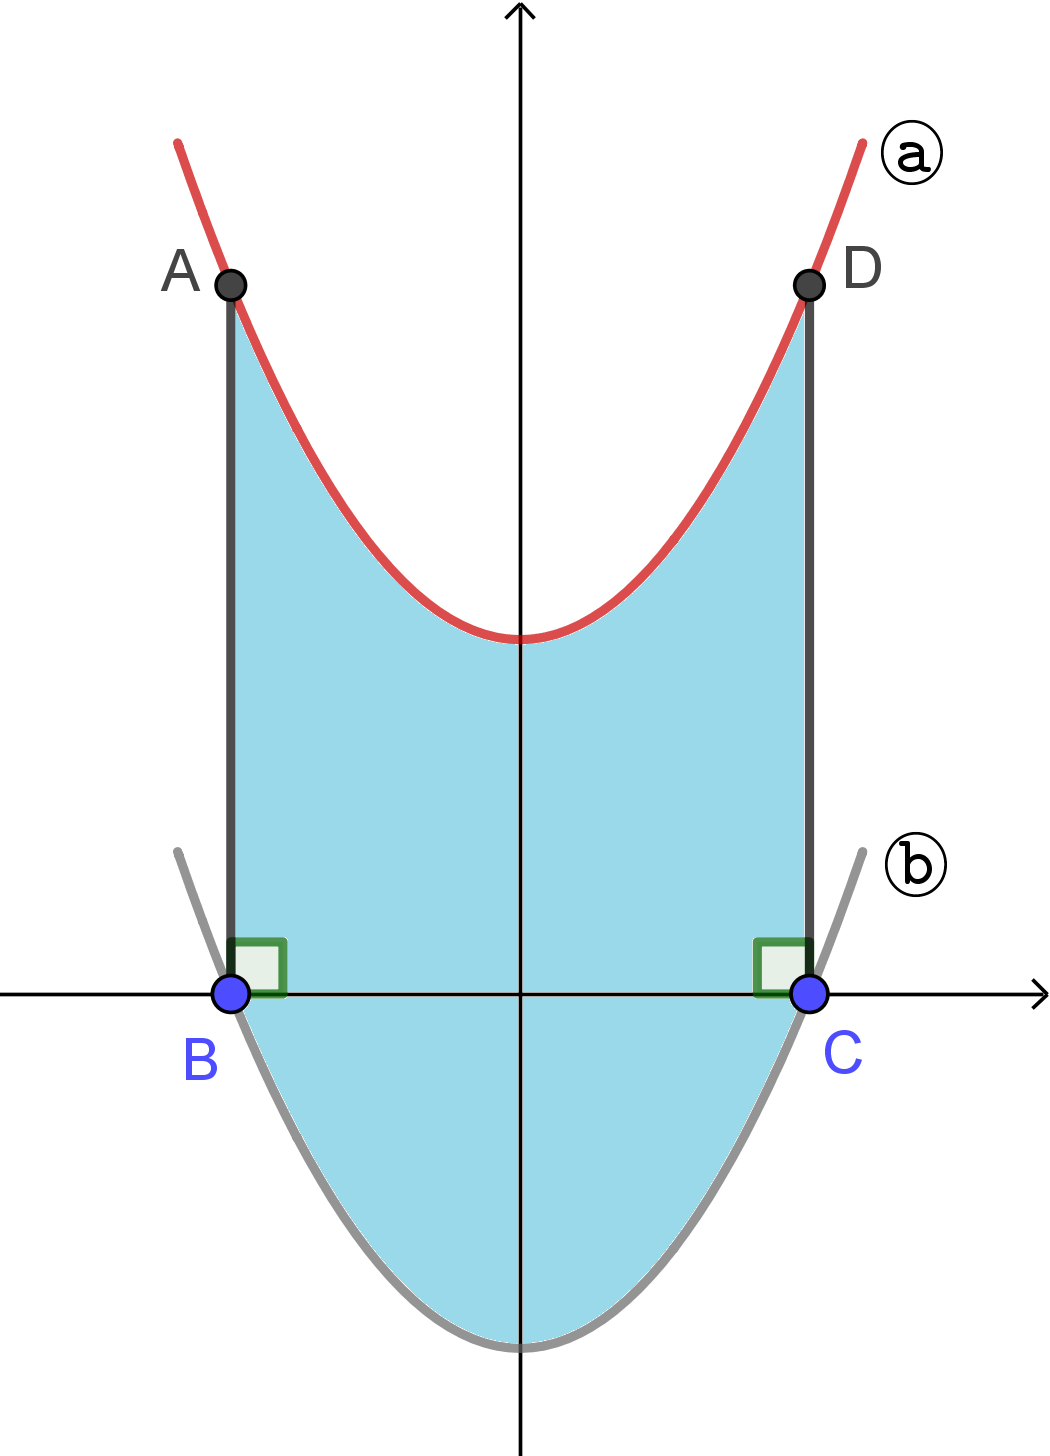
\includegraphics[width=0.23\textwidth]{130_2}
\end{center}
\taba{3\sqrt3}{6\sqrt3}{3\sqrt6}{6\sqrt6}{12\sqrt6}

\newpage
%
\prob{130-3}\label{130-3}%1
아래 그림에서 ⓐ, ⓑ는 각각 이차함수 \(y=x^2\)와 \(y=(x-2)^2\)의 그래프이다.
이때, 색칠한 부분의 넓이를 구하여라.
\begin{center}
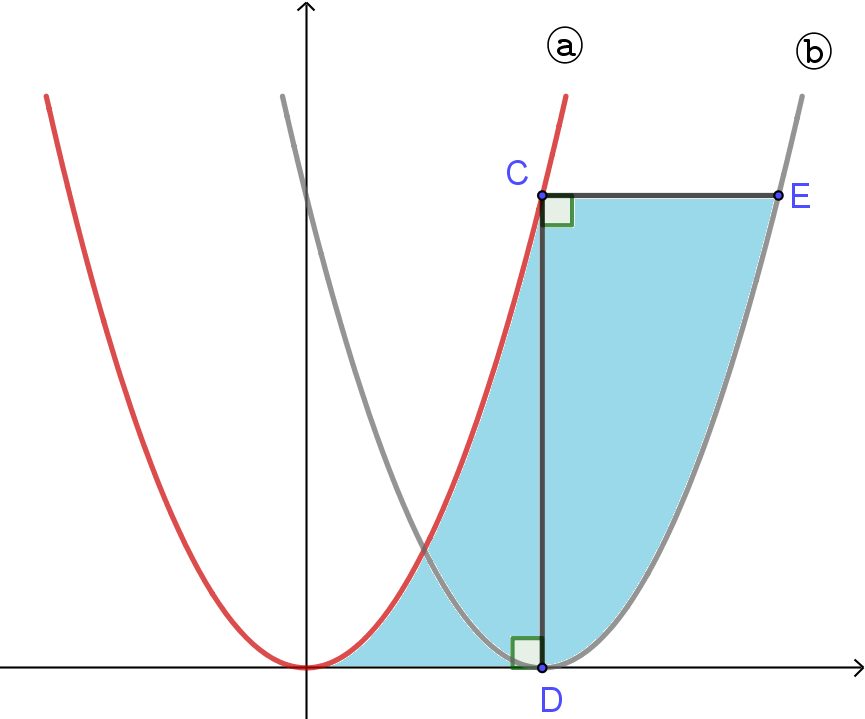
\includegraphics[width=0.3\textwidth]{130_3}
\end{center}
\taba8{12}{16}{20}{24}

%
\prob{133-1}\label{133-1}%5
이차함수 \(y=ax^2+bx+c\)의 그래프가 두 점 \((1,4)\), \((5,4)\)를 지날 때, 이 이차함수의 그래프의 축의 방정식을 구하여라.
\tabb{x=-1}{x=0}{x=1}{x=2}{x=3}

%
\prob{133-2}\label{133-2}%4
이차함수 \(y=ax^2+bx+c\)의 그래프가 두 점 \((-2,-2)\), \((6,-2)\)를 지날 때, 이 이차함수의 그래프의 축의 방정식을 구하여라.
\tabb{x=-1}{x=0}{x=1}{x=2}{x=3}

%
\prob{142-1}\label{142-1}%4%a=3,b=6
이차함수 \(y=-x^2-(a+5)x-10\)는 \(x=-4\)에서 최댓값 \(b\)을 가진다.
이때, \(a+b\)의 값을 구하여라.
\taba0369{12}

%
\prob{142-2}\label{142-2}%2%a=2,b=1
이차함수 \(y=x^2-2x+3a-1\)는 \(x=b\)에서 최솟값 \(4\)을 가진다.
이때, \(a+b\)의 값을 구하여라.
\taba0369{12}

%
\prob{143-1}\label{143-1}%k=2
이차함수 \(y=-\frac13x^2+kx\)의 최댓값이 \(3\)일 때, 상수 \(k\)의 값을 구하여라.
(단, \(k>0\))
\taba12345

%
\prob{143-2}\label{143-2}%k=3
이차함수 \(y=2x^2+(k+5)x\)의 최솟값이 \(-8\)일 때, 상수 \(k\)의 값을 구하여라.
(단, \(k>0\))
\taba12345

%
\prob{143-3}\label{143-3}%k=3
이차함수 \(y=-x^2+6x+2k-10\)의 꼭짓점이\\
\(3x-y=4\) 위에 있을 때, 이 이차함수의 최솟값을 구하여라.
(단, \(k\)는 상수)
\taba12345

%
\prob{143-4}\label{143-4}%k=4
이차함수 \(y=0.02x^2+\frac2{25}x+\frac k{20}\)의 꼭짓점이\\
\(x+100y=10\) 위에 있을 때, 이 이차함수의 최솟값을 구하여라.
(단, \(k\)는 상수)
\taba12345

\newpage
%
\prob{144-1}\label{144-1}%1
어느 떡집의 \(1000\)원짜리 떡은 하루에 400개씩 팔리는데, 이 떡의 가격을 \(x\)원 내리면 판매량이 \(2x\)만큼 늘어난다고 한다.
이때, 총판매 금액이 최대가 되도록 하려면 개당 가격을 얼마로 정해야 하는가?
\tabb{600원}{700원}{800원}{900원}{1000원}

%
\prob{144-2}\label{144-2}%1
어느 상점에서 한 자루에 \(600\)원인 볼펜이 하루에 \(100\)자루가 팔리는데, 이 볼펜의 가격을 \(10\)원씩 내릴 떄마다 판매량이 \(2\)자루씩 늘어난다고 한다.
이때, 총 판매 금액이 최대가 되도록 하려면 볼펜의 가격을 얼마로 정해야 하는가?
\tabb{550원}{560원}{570원}{580원}{590원}

%
\prob{145-1}\label{145-1}%4%54
점 \(A(0,12)\)와 이차함수 \(y=\frac13x^2\)의 그래프 위의 점 \(B\)를 이은 선분 \(AB\)가 \(x\)축과 평행하다.
아래 그림과 같이 \(\square ABCD\)가 평행사변형이 되도록 두 점 \(C\), \(D\)를 \(y=\frac13x^2\)의 그래프 위에 잡을 때, 평행사변형의 넓이를 구하여라.
\begin{center}
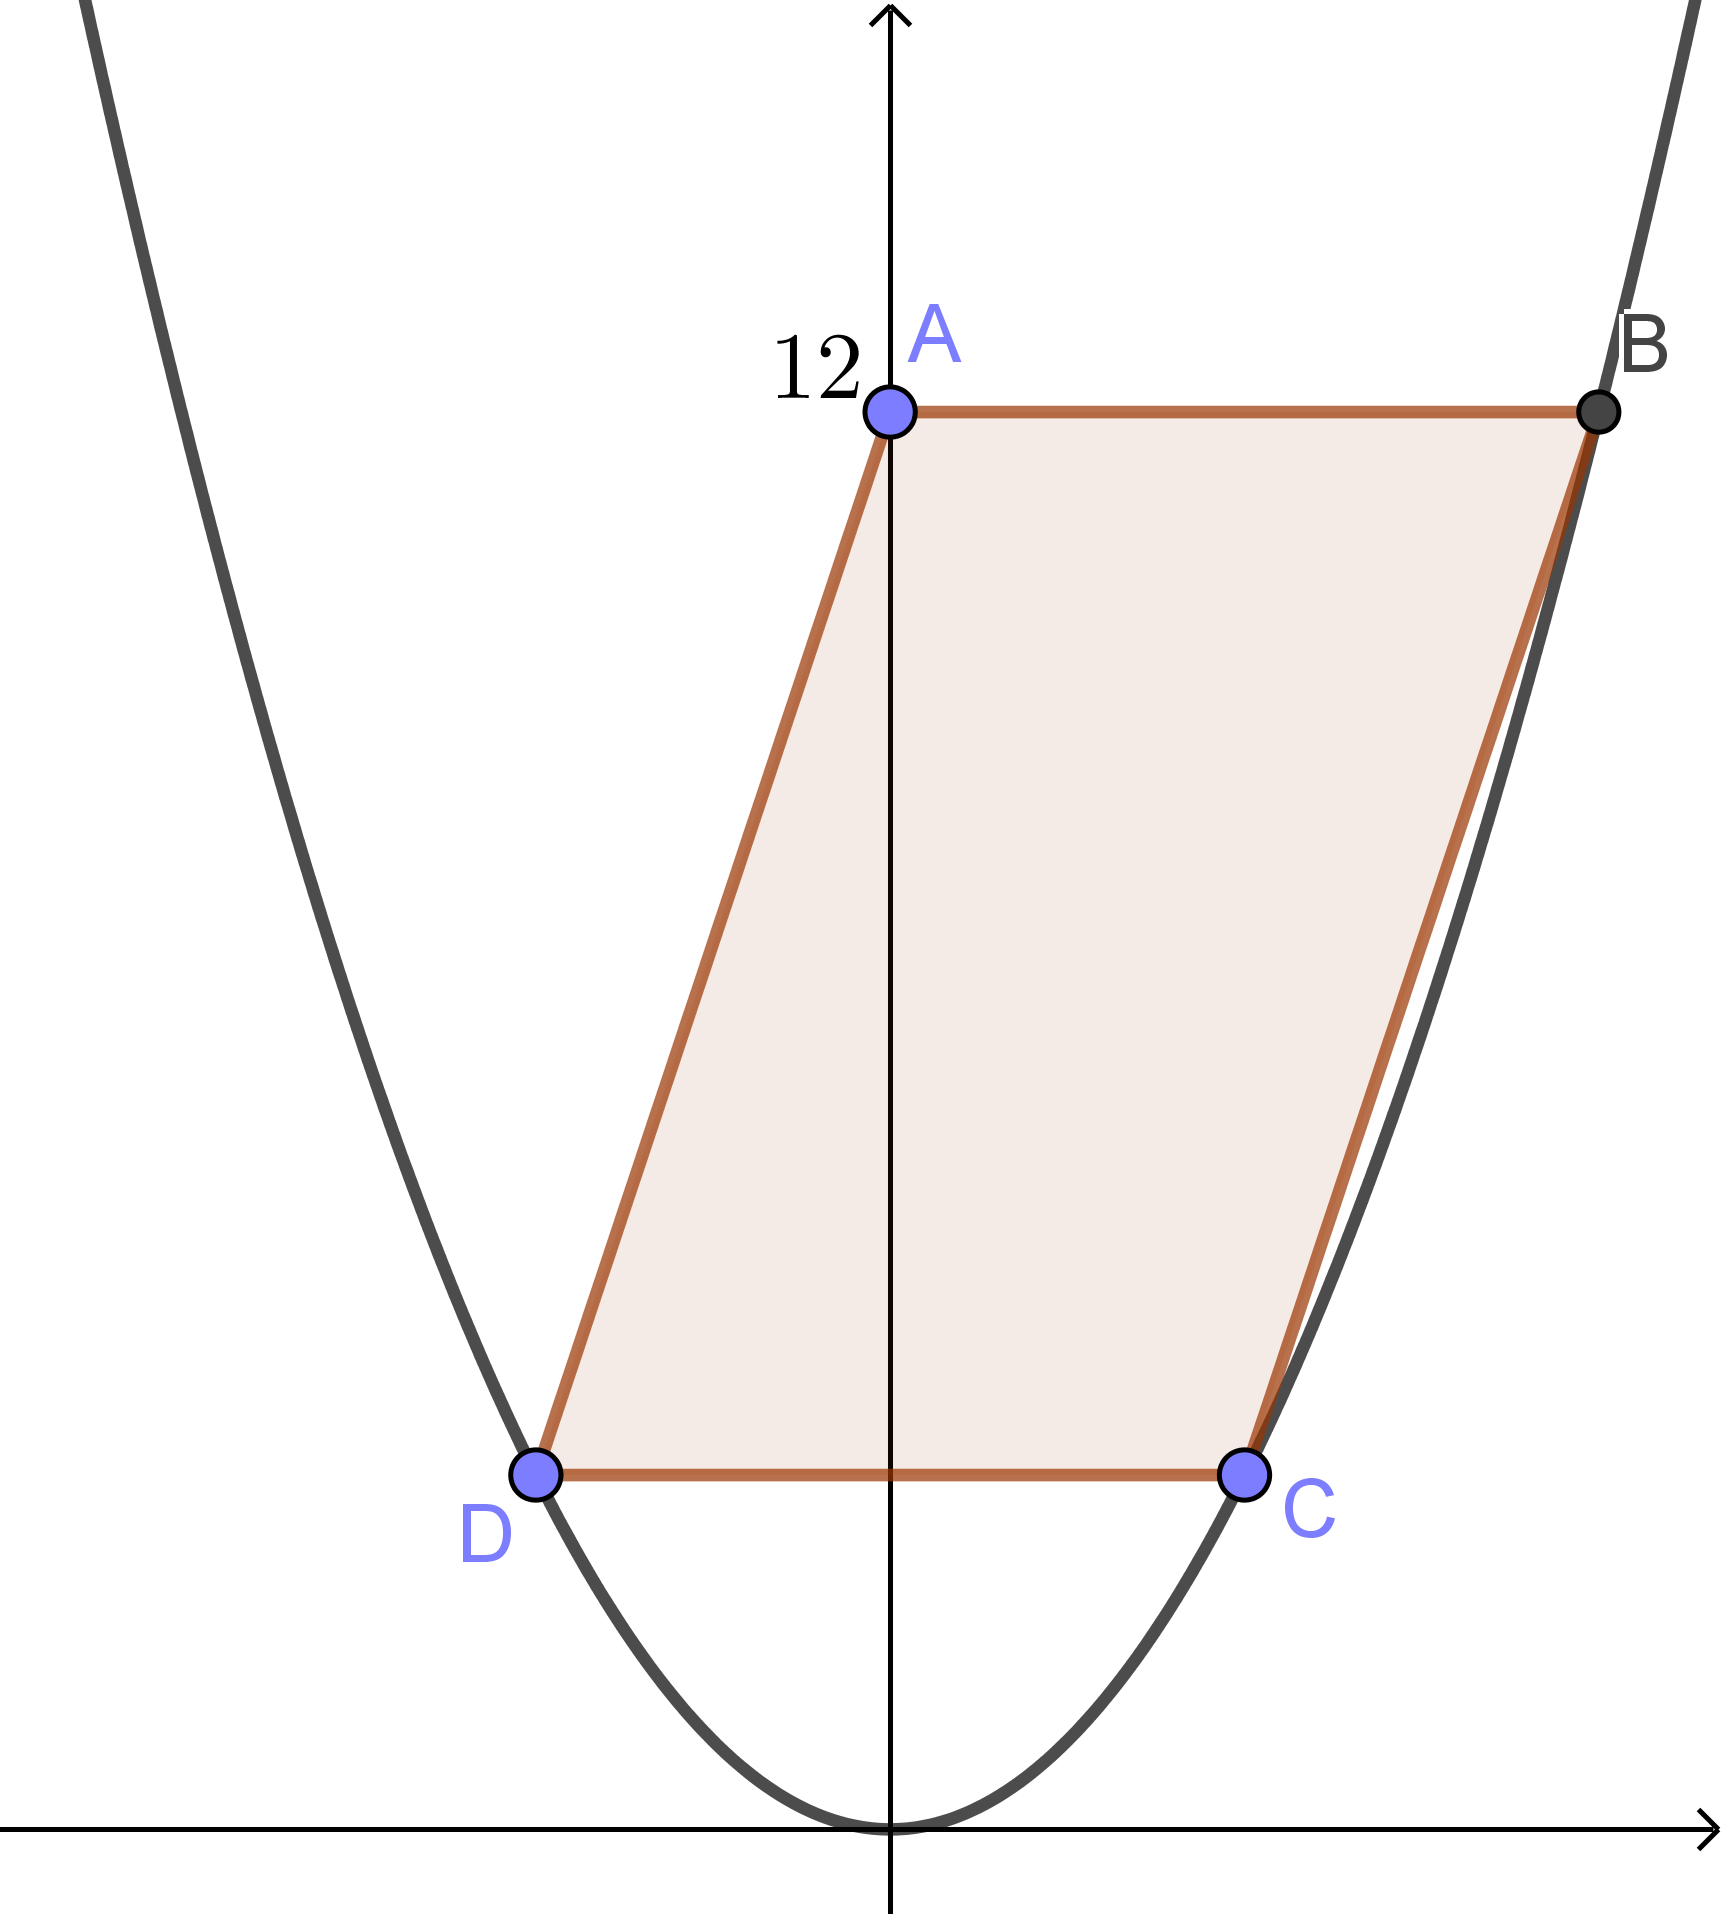
\includegraphics[width=0.2\textwidth]{145_1}
\end{center}
\taba{48}{50}{52}{54}{56}

\newpage
%
\prob{145-2}\label{145-2}%1%48
점 \(A(0,16)\)와 이차함수 \(y=x^2\)의 그래프 위의 점 \(B\)를 이은 선분 \(AB\)가 \(x\)축과 평행하다.
아래 그림과 같이 \(\square ABCD\)가 평행사변형이 되도록 두 점 \(C\), \(D\)를 \(y=x^2\)의 그래프 위에 잡을 때, 평행사변형의 넓이를 구하여라.
\begin{center}
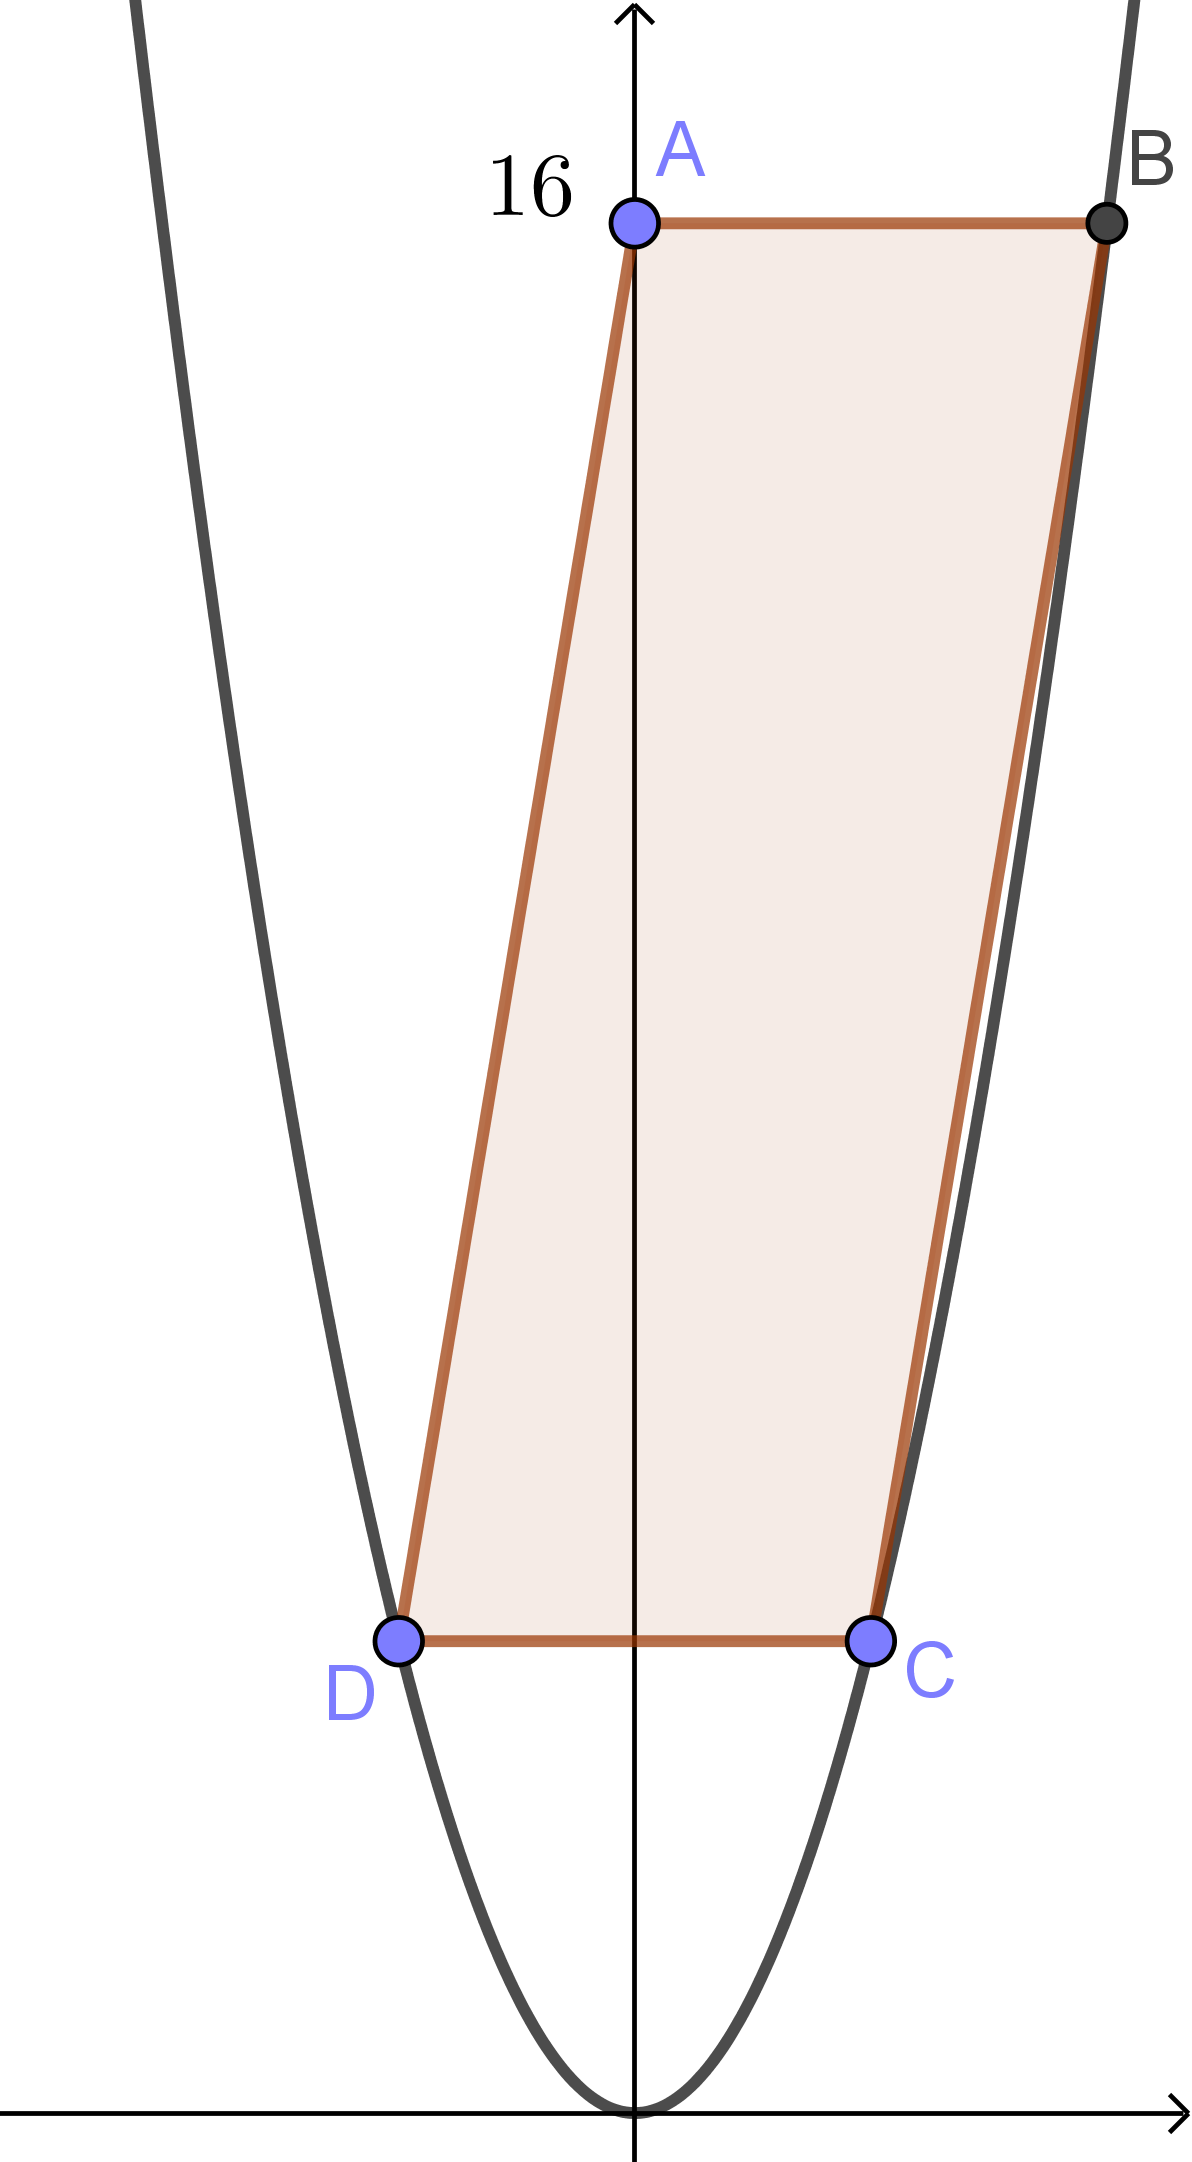
\includegraphics[width=0.2\textwidth]{145_2}
\end{center}
\taba{48}{50}{52}{54}{56}

\newpage
%
\prob{148-1}\label{148-1}%3
일차함수 \(y=-2x+12\)의 그래프 위의 한 점 \(P\)에서 \(x\)축, \(y\)축에 내린 수선의 발을 각각 \(Q\), \(R\)이라 할 때, 직사각형 \(ROQP\)의 넓이가 최대가 되도록 하는 점 \(P\)의 좌표는?
(단, 점 \(P\)는 제 1사분면 위의 점이다.)
\begin{center}
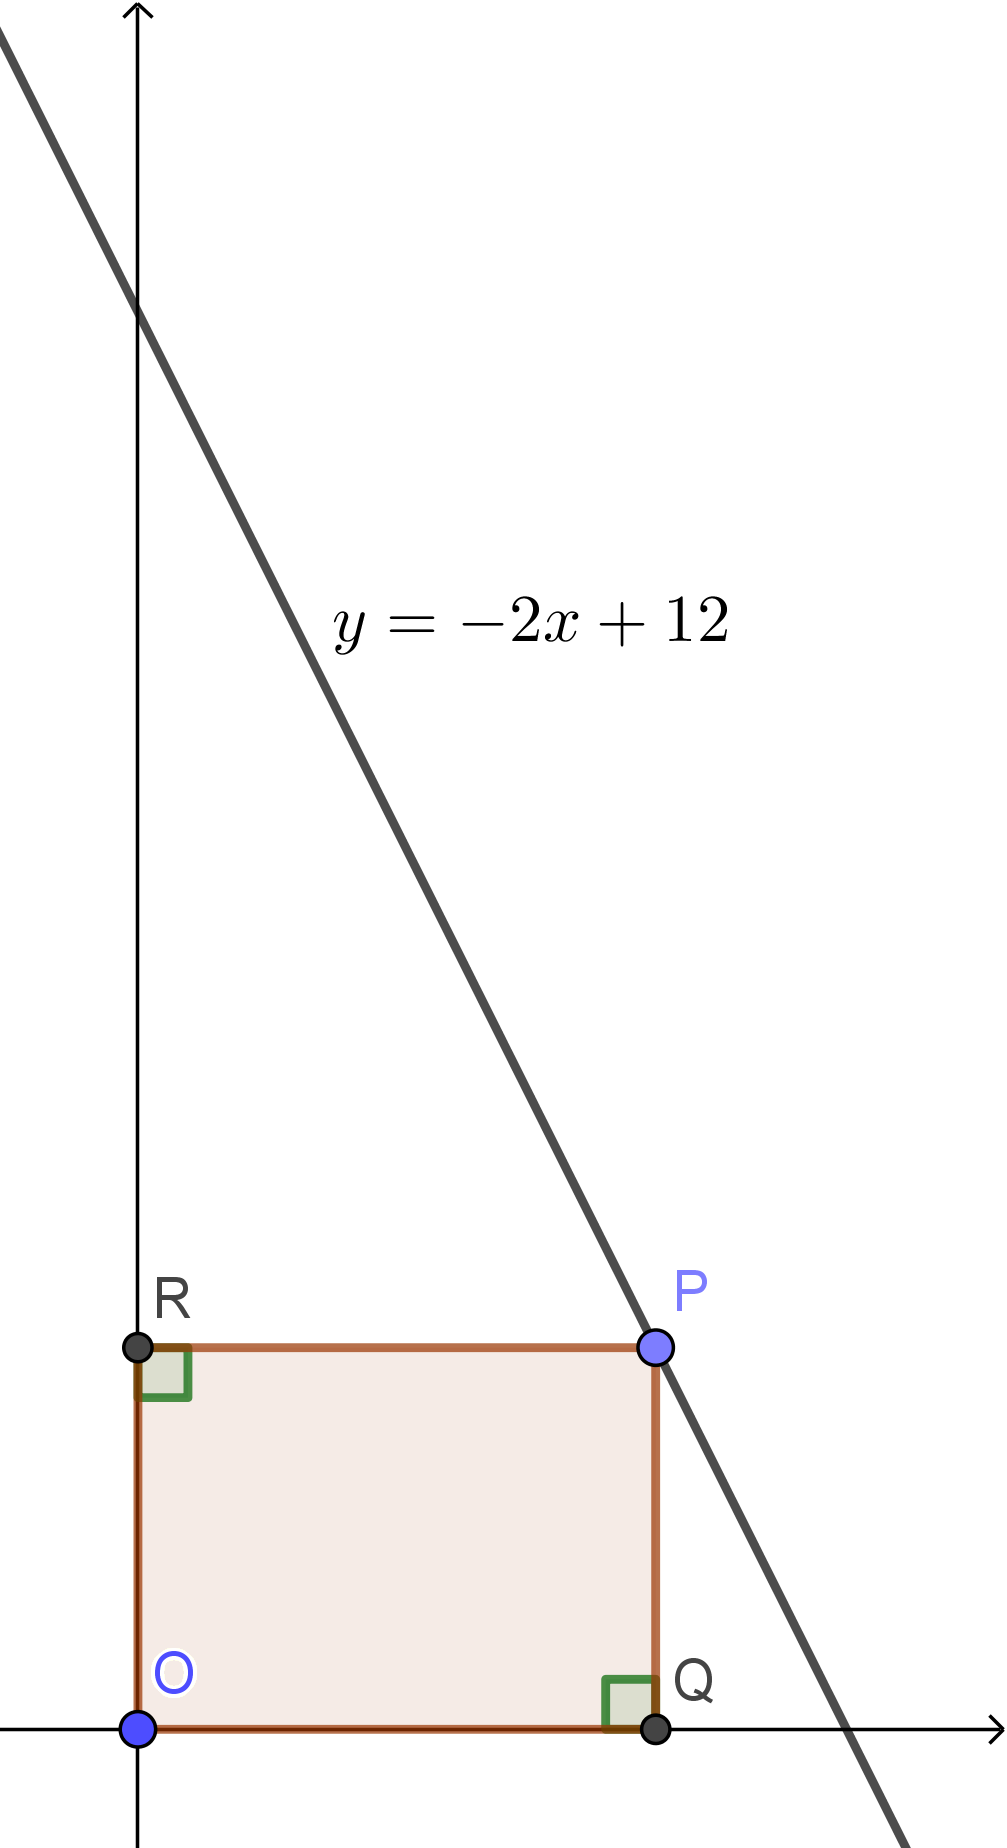
\includegraphics[width=0.2\textwidth]{148_1}
\end{center}
\tabb{(1,10)}{(2,8)}{(3,6)}{(4,4)}{(5,2)}

\newpage
%
\prob{148-2}\label{148-2}%1
직선 \(y=-2x+4\) 위를 움직이는 점 \(P\)가 있다.
점 \(P\)는 제 1사분면 위의 점이고 점 \(Q\)는 점 \(P\)에서 \(x\)축에 내린 수선의 발일 때, \(\triangle POQ\)의 넓이의 최댓값을 구하여라.
\begin{center}
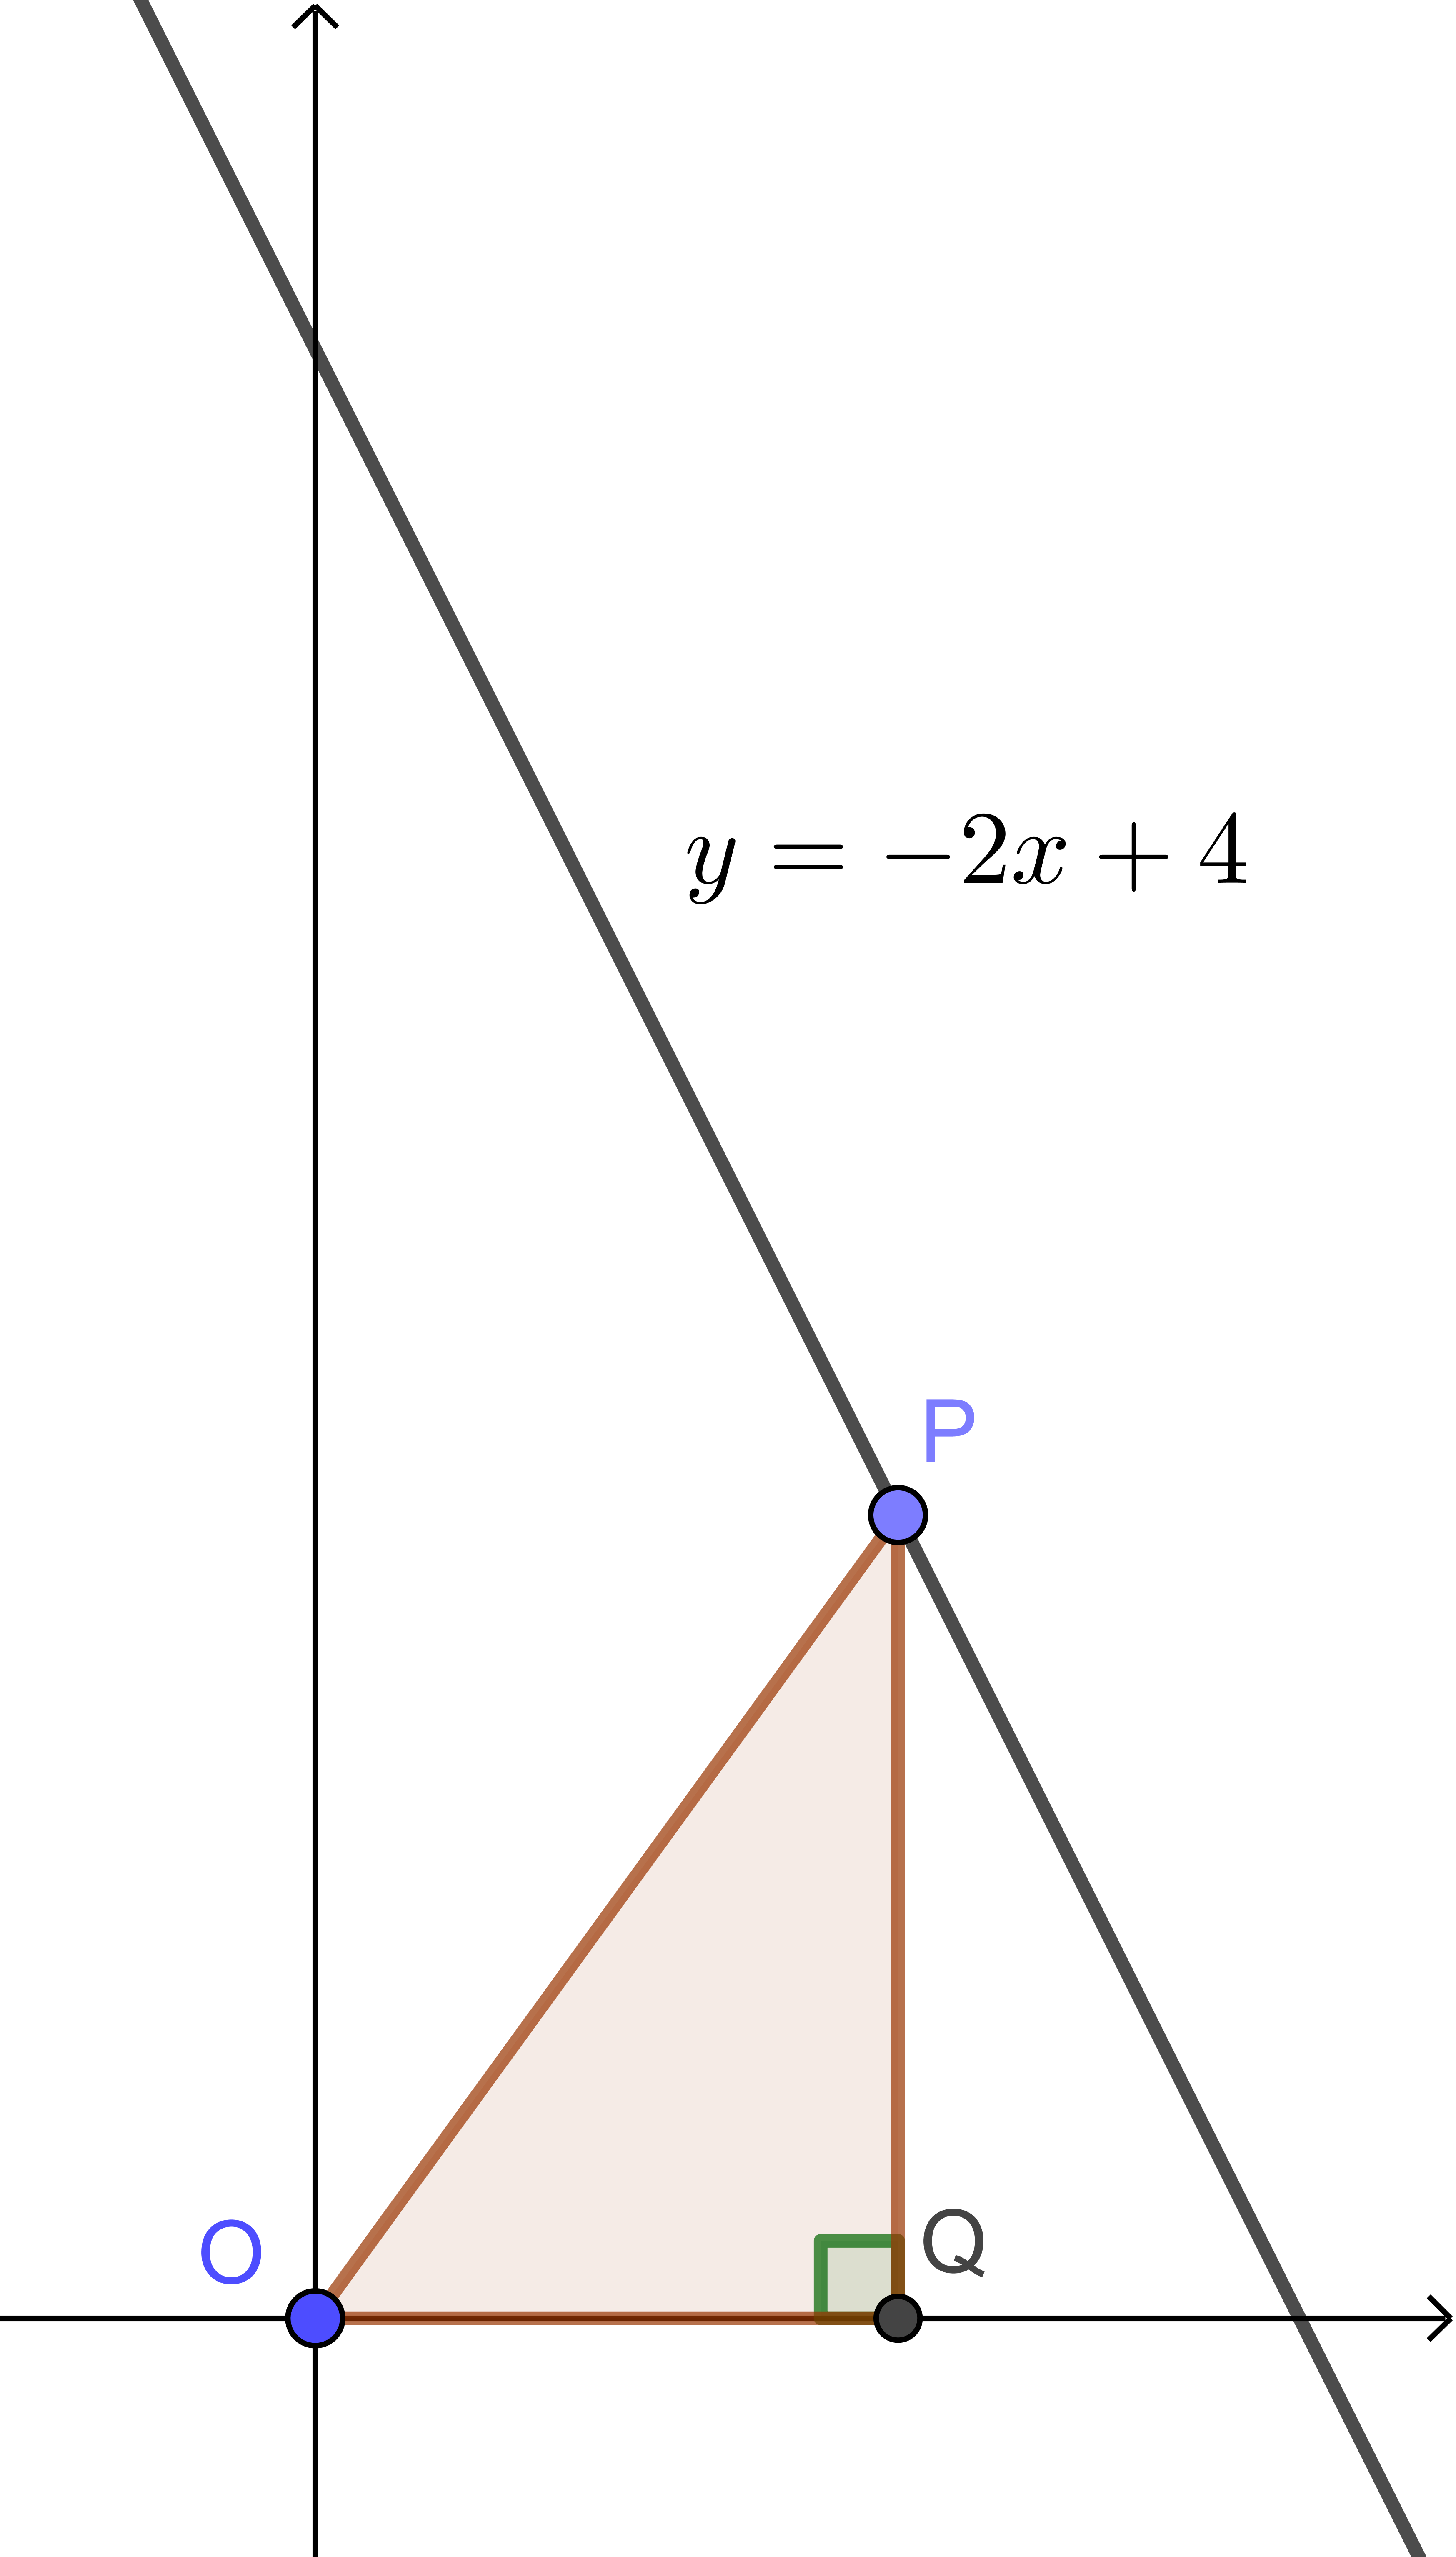
\includegraphics[width=0.2\textwidth]{148_2}
\end{center}
\taba12345

\newpage
%%
\section*{답}

\an{78}\four
\an{82-1}\two
\an{82-2}\one
\an{82-3}\three
\an{86-1}\(x=3\)\par\vspace{-30pt}
\begin{center}
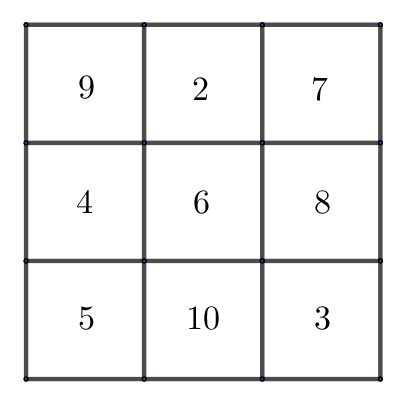
\includegraphics[width=0.2\textwidth]{86_1a}
\end{center}
\an{86-2}\(x=2\)\par\vspace{-30pt}
\begin{center}
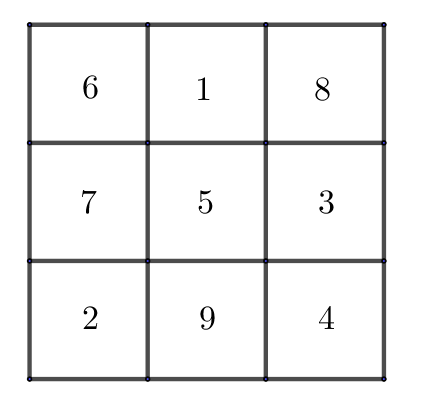
\includegraphics[width=0.2\textwidth]{86_2a}
\end{center}
\an{86-3}\(x=4\)\par\vspace{-30pt}
\begin{center}
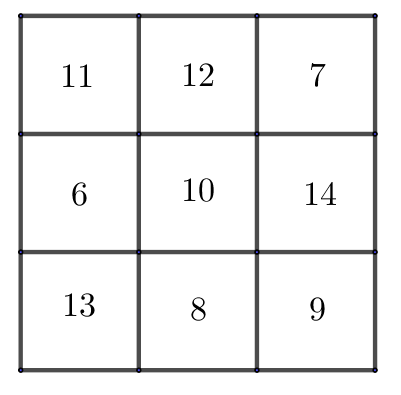
\includegraphics[width=0.2\textwidth]{86_3a}
\end{center}

\newpage
\begin{minipage}{0.2\textwidth}
\an{92-1}\one
\an{92-2}\three
\an{92-3}\five
\an{92-4}\one
\an{92-5}\two
\an{92-6}\five
\an{98-1}\two
\an{98-2}\four
\an{101-1}\four
\an{101-2}\two
\end{minipage}
\begin{minipage}{0.2\textwidth}
\an{101-3}\five
\an{101-4}\four
\an{101-5}\three
\an{102-1}\one
\an{102-2}\three
\an{103-1}\four
\an{103-2}\two
\an{106-1}\four
\an{106-2}\one
\an{106-3}\one
\an{107-1}\four
\end{minipage}
\begin{minipage}{0.2\textwidth}
\an{107-2}\four
\an{107_3}\four
\an{123-1}\three
\an{123-2}\two
\an{123-3}\one
\an{130-1}\five
\an{130-2}\five
\an{130-3}\one
\an{133-1}\five
\an{133-2}\four
\an{142-1}\four
\end{minipage}
\begin{minipage}{0.2\textwidth}
\an{142-2}\two
\an{143-1}\two
\an{143-2}\three
\an{143-3}\three
\an{143-4}\four
\an{144-1}\one
\an{144-2}\one
\an{145-1}\four
\an{145-2}\one
\an{148-1}\three
\an{148-2}\one
\end{minipage}

\end{document}